\documentclass{tufte-book}

\hypersetup{colorlinks}

\title[PETSc for PDEs]{PETSc \\ for \\ Partial \\ Differential \\ Equations}
\author{Ed Bueler}
\publisher{Maybe Someday a Publisher of This Book}

\date{\today}

\usepackage{booktabs} % for nicely-typeset tabular material
\usepackage{verbatim} % for "comment" environment
\usepackage{xspace}
%\usepackage{underscore} % causes "Missing \endcsname inserted" error?
\usepackage{fancyvrb}
\usepackage{graphicx}
\usepackage{amsmath,amssymb,amsthm,bm}
\usepackage{tikz}
\usetikzlibrary{arrows,decorations.markings}

%\usepackage[subtle,floats]{savetrees}

% macros

\theoremstyle{definition}
\newtheorem*{example}{{\color{cyan} Example}}

\newcommand{\trueinput}[2]{
\VerbatimInput[frame=single,framesep=3mm,label=\fbox{\normalsize \textsl{\,#1\,}},fontfamily=courier,fontsize=\footnotesize]{#2}
}

%\inputfromline{FULLPATH}{FILENAME}{CAPTION}{FIRSTLINE}{LABEL}
\newcommand{\inputfromline}[5]{
\vspace{0.8cm}
\let\FancyVerbStartString\relax
\let\FancyVerbStopString\relax
\begin{minipage}[l]{1.25\textwidth}
\VerbatimInput[frame=single,%
               framesep=3mm,%
               label=\fbox{\small \textsl{\,#2\,}},%
               fontfamily=courier,%
               fontsize=\scriptsize,%
               firstline=#4]{#1}
\end{minipage}
\vspace{0.5cm}

\begin{marginfigure}[1.0cm]
\caption{#3}
\label{#5}
\end{marginfigure}

\vspace{1.5cm}
}

\newcommand{\inputwhole}[4]{\inputfromline{#1}{#2}{#3}{1}{#4}}

%\cinputraw{FULLPATH}{FILENAME}{CAPTION}{PARTSTRING}{STARTSTRING}{STOPSTRING}{LABEL}
\newcommand{\cinputraw}[7]{
\newcommand*\FancyVerbStartString{#5}
\newcommand*\FancyVerbStopString{#6}
\vspace{0.8cm}
\begin{minipage}[l]{1.25\textwidth}
\VerbatimInput[frame=single,%
               framesep=3mm,%
               label=\fbox{\small \textsl{\,#2\,}#4},%
               fontfamily=courier,%
               fontsize=\scriptsize]{#1}
\end{minipage}
\vspace{0.5cm}

\begin{marginfigure}[1.0cm]
\caption{#3}
\label{#7}
\end{marginfigure}

\vspace{1.5cm}
\let\FancyVerbStartString\relax
\let\FancyVerbStopString\relax
}

\newcommand{\cinput}[5]{%
    \cinputraw{cstrip/#1}{#1}{#2}{}{#3}{#4}{#5}}
\newcommand{\cinputnostrip}[5]{%
    \cinputraw{../c/#1}{#1}{#2}{}{#3}{#4}{#5}}

\newcommand{\cinputpart}[6]{%
    \cinputraw{cstrip/#1}{#1}{#2}{\quad \textbf{part #3}}{#4}{#5}{#6}}
\newcommand{\cinputpartnostrip}[6]{%
    \cinputraw{../c/#1}{#1}{#2}{\quad \textbf{part #3}}{#4}{#5}{#6}}

\newcommand{\caveat}[1]{\marginnote{\textsc{Where we stand:}\\  #1}}

% Prints an epigraph and speaker in sans serif, all-caps type.
\newcommand{\openepigraph}[2]{%
  %\sffamily\fontsize{14}{16}\selectfont
  \begin{fullwidth}
  \sffamily\large
  \begin{doublespace}
  \noindent\allcaps{#1}\\% epigraph
  \noindent \Large \allcaps{#2}% author
  \end{doublespace}
  \end{fullwidth}
}

\newcommand{\monthyear}{%
  \ifcase\month\or January\or February\or March\or April\or May\or June\or
  July\or August\or September\or October\or November\or
  December\fi\space\number\year
}

\newcommand{\bA}{\mathbf{A}}
\newcommand{\bB}{\mathbf{B}}
\newcommand{\bE}{\mathbf{E}}
\newcommand{\bF}{\mathbf{F}}
\newcommand{\bJ}{\mathbf{J}}

\newcommand{\bb}{\mathbf{b}}
\newcommand{\bn}{\mathbf{n}}
\newcommand{\bq}{\mathbf{q}}
\newcommand{\br}{\mathbf{r}}
\newcommand{\bu}{\mathbf{u}}
\newcommand{\bv}{\mathbf{v}}
\newcommand{\bw}{\mathbf{w}}
\newcommand{\bx}{\mathbf{x}}
\newcommand{\by}{\mathbf{y}}

\newcommand{\CC}{\mathbb{C}}
\newcommand{\RR}{\mathbb{R}}
\newcommand{\ZZ}{\mathbb{Z}}

\newcommand{\X}{\times}  % for nonzero entries in matrices
\newcommand{\redX}{{\color{red} \bm{\underline{\X}}}}
\newcommand{\blueX}{{\color{blue} \bm{\underline{\X}}}}

\newcommand{\XX}{$\bm{\times}$}  % for ticks in tables
\newcommand{\gX}{{\color{Gray} $\times$}}

\newcommand{\eps}{\epsilon}
\newcommand{\lam}{\lambda}
\newcommand{\lap}{\triangle}

\newcommand{\Div}{\ensuremath{\nabla\cdot}}
\newcommand{\Curl}{\ensuremath{\nabla\times}}
\newcommand{\grad}{\nabla}

\newcommand{\ip}[2]{\ensuremath{\left<#1,#2\right>}}

\newcommand{\cond}{\operatorname{cond}}
\newcommand{\onull}{\operatorname{null}}
\newcommand{\rank}{\operatorname{rank}}
\newcommand{\range}{\operatorname{range}}
\newcommand{\Span}{\operatorname{span}}

\renewcommand{\Re}{\operatorname{Re}}
\renewcommand{\Im}{\operatorname{Im}}

\newcommand{\Th}{\mathcal{T}_h}
\newcommand{\Pone}{\mathbf{P}_1}

\newcommand{\Matlab}{\textsc{Matlab}\xspace}
\newcommand{\Triangle}{\textsc{triangle}\xspace}
\newcommand{\MPI}{\textsc{MPI}\xspace}

\newcommand{\PETSc}{\textsc{PETSc}\xspace}

\newcommand{\pDM}{\texttt{DM}\xspace}

\newcommand{\pDMDA}{\texttt{DMDA}\xspace}
\newcommand{\pDMPlex}{\texttt{DMPlex}\xspace}
\newcommand{\pKSP}{\texttt{KSP}\xspace}
\newcommand{\pMat}{\texttt{Mat}\xspace}
\newcommand{\pSNES}{\texttt{SNES}\xspace}
\newcommand{\pTS}{\texttt{TS}\xspace}
\newcommand{\pVec}{\texttt{Vec}\xspace}
\newcommand{\pVecs}{\texttt{Vec}s\xspace}

%\renewcommand\floatpagefraction{.9}  %???

% eventually this is a good idea:
%\usepackage{makeidx}
%\makeindex

\begin{document}

% epigraph page first
\newpage\thispagestyle{empty}
\openepigraph{%
\dots when there are disputes among persons, we can simply say: Let us calculate, without further ado, to see who is right.
}{Gottfried Wilhelm Leibniz}
\vfill
\openepigraph{%
Developing parallel, nontrivial PDE solvers that deliver high performance is still difficult and requires months (or even years) of concentrated effort.  PETSc is a toolkit that can ease these difficulties and reduce the development time, but it is not a black-box PDE solver, nor a silver bullet
}{Barry Smith}
\vfill
\openepigraph{%
Tufte's style is known for its extensive use of sidenotes, tight integration of graphics with text, and well-set typography.
}{The Tufte-LaTeX\ Developers}
\vfill

\frontmatter

\maketitle

% v.4 copyright page
\newpage
\begin{fullwidth}
~\vfill
\thispagestyle{empty}
\setlength{\parindent}{0pt}
\setlength{\parskip}{\baselineskip}
Copyright \copyright\ \the\year\ \thanklessauthor

\par\smallcaps{Published by \thanklesspublisher}

%\par I have no idea if I should license this at this stage

\par\textit{First printing, \monthyear}
\end{fullwidth}

\tableofcontents

\begin{comment}
% dedication
\cleardoublepage
~\vfill
\begin{doublespace}
\noindent\fontsize{18}{22}\selectfont\itshape
\nohyphenation
Thanks to \mbox{Jed Brown} and \mbox{Constantine Khroulev}, fellow students, and gurus.
\end{doublespace}
\vfill
\end{comment}

%%%%%%%%%%

\chapter{Why this book?}


You've taken a mathematics course or two in partial differential equations (PDEs).  Somewhere you picked up a bit of coding in C; perhaps you write C code every day.\sidenote{You know that ``API'' stands for ``application program interface,'' for example.}  You've also written various short scripts in \Matlab or python, and you've even tried solving PDEs numerically.  But \emph{now you want it all in parallel on big problems}.  This book is for you and me.

\section{\PETSc?}

The Portable, Extensible Toolkit for Scientific computing (\PETSc\sidenote{Say it ``pets sea.''}) \citep{petsc-user-ref} is an open-source, mathematical software library built on top of the standard software layer for large-scale parallel computation, the Message Passing Interface (MPI) \citep{Groppetal1999}.  Thus \PETSc is a framework for solving problems like PDS at ``large scale,'' that is, at high resolution and on supercomputers with hundreds to millions of cores.

\PETSc is not particularly new.  Version 2.0, the first version to make an impact in the scientific computing world, was built in 1994.  A well-known textbook \citet{Smithetal1996}\sidenote{B.~Smith, P.~Bjorstad, and W.~Gropp. \emph{Domain decomposition: parallel multilevel methods for elliptic partial differential equations}. Cambridge
University Press, 1996} uses \PETSc 2.0 for scalable solutions of linear partial differential equations (PDEs).  That book focusses on pre-conditioned iterative linear solvers.  For example, domain decomposition methods like additive Schwarz are shown to scalably solve the Poisson equation on irregular domains and fine meshes in parallel.

But \PETSc is now at version 3.5.\sidenote{Version 3.5.2 is current in September 2014.  The stable homepage URL for PETSc, including download and installation instructions, is at \href{http://www.mcs.anl.gov/petsc/index.html}{www.mcs.anl.gov/petsc}.}  It has evolved into a more powerful toolbox with a much richer API.

Typical examples and applications now solve nonlinear PDEs at scale.  The \PETSc strategy is to compose Newton's method and mesh topology tools with a run-time chooseable selection of preconditioners and iterative linear solvers.  The nonlinear and multilevel-related parts of the \PETSc API are now highly-visible to users of \PETSc 3.5.  ``Multiphysics problems''\sidenote{This buzzword just refers to a diverse system of coupled PDEs with nontrivial scalings among the variables.  But that is a concept that \emph{needs} a buzzword.} are now within reach.  \PETSc may not be a silver bullet, but users see powerful tools, beyond linear algebra, to solve hard problems.

On the other hand, \PETSc is notoriously complicated.  Twenty years have passed since \PETSc version 2.0.  Perhaps a new book is needed.

\section{The goals of this book}

This book is about approximately solving linear and nonlinear PDEs in 2 or 3 spatial variables by writing C code that calls \PETSc methods.  It tries to both explain the ideas directly, and illustrate them through example codes.  The example codes come with enough background information so that readers can use them as a basis for further developments.  Demonstrated scalability of these examples is the goal, so runtime options are explained and compared.

This book does not replace the \PETSc \emph{User's Manual}.  Indeed, the current book assumes you want to solve PDEs, while there are many other uses of \PETSc.

This book is written from the conviction that better access to common knowledge among experts advances scientific computing as a discipline.  In fact, accessing common knowledge advances the discipline faster than does original research among the experts.  Said another way, I hope that an expert in \PETSc will say about this book's content that ``I knew all that'' \emph{and} that ``this book is a fast on-ramp to what I already know.''

\section{What I need from you, the reader}

To make sense of this book, some of the mathematical theory\sidenote{\citep{Evans} is recommended, but not really a prerequisite.} of PDEs must be familiar.  I will also assume some nebulous, and hard to define, practical intuition about PDE problems, including exposure to nonlinear ones.\sidenote{\citep{Ockendonetal2003} is recommended.}  Of course, all applied mathematicians, distinctly including this author, are wanting when it comes to injesting the mathematical theory of, and building intuition for, nonlinear PDEs.

Multiple numerical discretization paradigms for PDEs will arise in this book.  At least one such numerical approach to PDEs should be in the reader's toolbox.  This background might be based on the finite element method (FEM) \citep{Braess,Elmanetal2005}, finite differences \citep{MortonMayers}, finite volumes \citep{LeVeque}, or spectral methods \citep{KarniadakisSherwin,Trefethen}.  Exposure to multigrid ideas \citep{Briggsetal2000} would be helpful, but these concepts will be reviewed.  Numerical ideas from linear algebra \citep{Greenbaum1997,TrefethenBau} will also appear, often with only a brief introduction.

Starting in Chapter 3 I will assume that you are at least a bit interested in applying the finite element method (FEM) on unstructured grids, though not at the exclusion of structured approaches.  The basics of the FEM method will be reviewed, but the reader must also bring some background understanding of this nontrivial topic.  Perhaps the weak form of a PDE, and the idea of assembling the systems of equations element-by-element, are ``rusty'' topics.  But these topics should be in there somewhere.

Searching in the \PETSc HTML manual pages should be the reader's first resort for resolving compile-time errors, or for exposing the \PETSc API.  However, the reader should also see which topics are addressed in the \PETSc \emph{Users Manual}.  That \emph{Manual} often explains why the API is designed in the way it is.


\section{There is much that this book does NOT do}

Here is a partial list:\begin{itemize}
\item This book does not help you install \PETSc.
\item This book does not replace \citep{Smithetal1996}.
\item This book does not do anything in Fortran.
\item This book does not help with most packages \PETSc links to.
\item This book does not do a complete job of teaching the finite element method.
\item This book does not solve any hyperbolic PDE problems.
\item This book does not consider spatial dimensions except 2 and 3.
\item This book does not prove anything.\sidenote{We do give evidence for convergence and scalability when possible.}
\item This book does not care whether its numerical solutions are good models of physical problems.
\item This book does not adequately cover what is known about nonlinear PDEs, much less what is not known.
\end{itemize}


\mainmatter

%%%%%%%%%


\chapter{Getting started with PETSc}
\label{chap:getstarted}

\section{A code that does almost nothing, but in parallel}

The purpose of the \PETSc library is to help you solve scientific and engineering problems, such as PDEs of course, on distributed computers.  But \PETSc is built ``on top of'' the Message Passing Interface (MPI; \citep{Groppetal1999}) library, and some of the flavor of that library comes through.  We start with an example C code that is essentially an introductory MPI example, though it calls \PETSc for some basic tasks.

This code \texttt{c1e.c}, shown in its entirety in Figure \ref{code:e}, computes Euler's constant
\begin{equation}
e = \sum_{n = 0}^\infty \frac{1}{n!} \approx 2.718281828 \label{introeseries}
\end{equation}
It does the computation in a distributed manner by computing one term of the infinite series on each process.  Thus it computes a better estimate of $e$ when run on more MPI processes. While this is a silly use of \PETSc, it is an easy to understand parallel computation.

As with any C source for an executable, \texttt{c1e.c} has a function called \texttt{main()} which takes inputs from the command line, namely \texttt{argc} and \texttt{argv},\sidenote{Here \texttt{argc} is an \texttt{int} holding the argument count.  The second argument \texttt{argv} is an array of strings (i.e.~C type \texttt{char**}) holding the command line (i.e.~command and arguments).  However, in all codes in this book we simply pass these arguments on to \PETSc through the \texttt{PetscInitialize()} method.} and which outputs an \texttt{int} which is $0$ if the program succeeds.  Also, like all C codes, we include the needed headers; only \texttt{petscsys.h} is needed here, but later codes will include other \PETSc headers.

The substance of \texttt{main()} is to declare some variables, do a computation on each process, and communicate the results between processes to get an estimate of $e$.  Finally we report success (i.e.~return $0$) at the end.

More details of \texttt{c1e.c} can be described once we compile and run the code.  Please do the following to start:
\begin{cline}
$ cd p4pdes/c/  # download this book, and its codes in p4pdes/c/, by
                #     "git clone https://github.com/bueler/p4pdes.git"
$ make c1e
\end{cline}
For the command ``\texttt{make}'' to work there must be a makefile, of course, and it is \texttt{/p4pdes/c/makefile}, shown in Figure \ref{code:c1emakefile}.  For all the codes in this book, the makefile will have this form, exactly as recommended in the \PETSc User's Manual \citep{petsc-user-ref}.

\inputwhole{../c/c1e.c}{\texttt{p4pdes/c/c1e.c}}{Compute $e$ in parallel.}{code:e}

Run the code on one MPI process like this:
\begin{cline}
$ ./c1e
e is about 1.000000000000000
rank 0 did 1 flops
\end{cline}
%$
The value $1.0$ is a very poor estimate of $e$, but this code does better with more processes:
\begin{cline}
$ mpiexec -n 5 ./c1e
rank 3 did 7 flops
rank 4 did 9 flops
e is about 2.708333333333333
rank 0 did 1 flops
rank 1 did 3 flops
rank 2 did 5 flops
\end{cline}
%$
That's a better estimate of $e$, but hardly impressive.  On the other hand, with $N=20$ processes, and thus $N=20$ terms in series \eqref{introeseries}, we get a good estimate:
\begin{cline}
$ mpiexec -n 20 ./c1e
rank 9 did 19 flops
...
e is about 2.718281828459045
rank 0 did 1 flops
...
rank 18 did 37 flops
\end{cline}
%$

\cinputraw{c1emakefile.frag}{extract from \texttt{p4pdes/c/makefile}}{All \texttt{makefile}s for the \PETSc codes in this book look like this.}{}{//START}{//STOP}{code:c1emakefile}

Now, perhaps the reader is worried that this book was written using a large supercomputer whereas the reader has a little laptop with only a couple of cores.  Not so; these $N=5$ and $N=20$ process MPI calls work just fine on the author's four-core laptop because MPI processes are created as needed.\sidenote{Multitasking operating systems have been around for quite some time!}

The main job in \texttt{c1e.c} is to collect the sum of the terms of (truncated) infinite series \eqref{introeseries} onto each process.  After each process computes term $1/n!$, where $n$ is its rank in the MPI communicator, a call to \texttt{MPI\_Allreduce()} does the sum and then sends the sum back to each process.  We also get the rank of the current process with a call to \texttt{MPI\_Comm\_rank()}.  These direct uses of the MPI library illustrate that \PETSc, which tries to avoid duplication of MPI functionality, need not be called for some low-level parallel tasks.

In \texttt{c1e.c} we print the computed estimate of $e$, and we also have each process print its rank and the work it did.  Observe that \texttt{PetscPrintf()}, a formatted print command like \texttt{fprintf()} from the C standard library, is called twice, once with MPI communicator \texttt{PETSC\_COMM\_WORLD} and once with \texttt{PETSC\_COMM\_SELF}.\sidenote{Thereby we illustrate collective and non-collective operations in the same program.}  The first of these \texttt{STDOUT} printing jobs is therefore \emph{collective} over all processes, and thus only done once, and other printing job is individual to each rank.\sidenote{A process is often just called a \emph{rank} in MPI language.}  In the output the \texttt{PETSC\_COMM\_SELF} printed lines appear in almost random order because the print occurs as soon as that process reaches that line.

Every \PETSc program should start and end with the commands \texttt{PetscInitialize()} and \texttt{PetscFinalize()}:
\begin{code}
PetscInitialize(&argc,&args,(char*)0,help);
... everything else goes here ...
PetscFinalize();
\end{code}
Also, so that this \PETSc code can provide useful usage help, we add a \texttt{help} string at the start; it is a good place to say what the purpose of the code is.

There is one more observation about \texttt{c1e.c} and all \PETSc programs: there is error-checking clutter from capturing and checking the return code of each method called.  While languages other than C could help with decluttering this stuff, we are stuck with lines that look like
\begin{code}
ierr = PetscCommand(...); CHKERRQ(ierr);
\end{code}
The explanation of this clutter is that almost all \PETSc methods, and most user-written methods in \PETSc programs, return an \texttt{int} for error checking, with value $0$ if successful.  In the line above, \texttt{ierr} is a \texttt{PetscInt} type and \texttt{CHKERRQ()} is a macro which does nothing if \texttt{ierr == 0} but which stops the program otherwise.  In the nonzero case the program stops with a traceback, namely a list of the nested methods, in reverse order, showing the line numbers and method names of the location where the error occurred.  This traceback tends to be the first line of defense when debugging run-time errors.  Examples in this book always capture-and-check the returned error code in this way, despite the clutter.  On the other hand, after this chapter we will strip the ``\texttt{ierr =}'' and ``\texttt{CHKERRQ(ierr);}'' clutter from the code displayed in the text, even though it is still present in the source file itself.


\section{Linear systems}

Of course, our goal in the remainder of the book is to compute more interesting quantities than Euler's constant $e$.  At the core of most \PETSc computations is a finite-dimensional linear system.  Before solving such systems in \PETSc, it is useful to recall the most basic ideas of numerical linear algebra.

Suppose $\bb\in \RR^{N}$ is a column vector and $A\in\RR^{N\times N}$ is a square matrix.  The linear system
\begin{equation}
A \bu = \bb \label{introsystem}
\end{equation}
has a unique solution if $A$ is invertible, namely
\begin{equation}
\bu = A^{-1} \bb. \label{introsolution}
\end{equation}
This is simple in theory.

It is not so simple in practice, however, when solving large systems on a computer.  There are two key facts to keep in mind while working numerically  \citep{TrefethenBau}.
\renewcommand{\labelenumi}{\roman{enumi})}
\begin{enumerate}
\item \emph{limit to accuracy}:  If real numbers are represented on the computer with machine precision $\eps$ then the solution of \eqref{introsystem} can only be computed within an error $\kappa(A) \eps$ where $\kappa(A) = \|A\|_2 \|A^{-1}\|_2$ is the (2-norm) \emph{condition number} of $A$.\sidenote{Fact i) is about \emph{conditioning} not \emph{methods}.  Informally speaking, there are linear systems $A,\bb$ that are the same to within $\eps$ but for which the infinite-precision solutions $\bu$ are different by the amount $\kappa(A) \eps$.}
\item \emph{cost of direct solutions}:  Computation of solution \eqref{introsolution} by a direct method like Gauss elimination, whether actually forming $A^{-1}$ or not, is an $O(N^3)$ operation.
\end{enumerate}

For a sense of the consequences of these facts, let's put in some numbers for $\eps$, $\kappa(A)$, and $N$.  On most computers the precision for the C \texttt{double} type, the modern default 64-bit representation of real numbers, is $\eps = 2.2 \times 10^{-16}$.  By i), a linear system having $\kappa(A) \approx 10^{10}$, for example, can only be solved to about six digits of precision.

Regarding computational cost, because of ii) a linear system with $N=10^6$ equations requires $\sim 10^{18}$ operations to solve by Gauss elimination.  While even modern supercomputers take a while to do a quintillion operations, so that Gauss elimination is impractical for systems of $N=10^6$ equations, we will successfully solve problems of this size on a single processor in a few seconds, and in $O(N)$ operations, in Chapter \ref{chap:multigrid}.
%time ./c4poisson -da_refine 7 -ksp_type cg -pc_type mg
%on 1153 x 1153 grid:  iterations 2, residual norm = 1.88082e-05
%real 11.18

To build our first \PETSc code for a linear system, we describe the \PETSc objects which store vectors and matrices.


\section{\PETSc \pVec and \pMat objects}

The \pVec object is a container and interface for a distributed vector, and a \pMat object holds a distributed matrix.  Although \PETSc is written in C, not C++, it is a relentlessly object-oriented software library.  Consider the operations which might touch a matrix object \texttt{A} in a linear system like \eqref{introsystem}:
\begin{code}
Mat A;
MatCreate(COMM,&A);
MatSetSizes(A,PETSC_DECIDE,PETSC_DECIDE,N,N);
PetscObjectSetName((PetscObject)A,"A");
MatSetOptionsPrefix(A,"a_");
MatSetFromOptions(A);
... fill entries of (i.e. assemble) A ...
... solve system with A ...
MatDestroy(&A);
\end{code}
In fact, for ``\pVec'' objects storing vectors, ``\pMat'' objects storing matrices, and indeed for all \PETSc object types, this basic sequence of operations applies:
\begin{code}
Object X;
ObjectCreate(COMM,&X);
... set properties of X from code ...
ObjectSetFromOptions(X);  // allows run-time setting of properties
... use X ...
ObjectDestroy(&X);
\end{code}
Of course ``\texttt{Object}'' here is merely a meta-name for a \PETSc type like \pVec or \pMat.

\PETSc objects are generically distributed across, and accessible from, multiple MPI processes.  Therefore the first argument of an \texttt{ObjectCreate()} method is an MPI communicator (``\texttt{COMM}'').  All processes in \texttt{COMM} must call the \texttt{ObjectCreate()} method.

Evidently \texttt{Mat A} above has an internal representation with nontrivial structure, but that is hidden.  Indeed the data structure inside \texttt{A} depends on runtime choices, the most basic being that the number of bytes used to store \texttt{A} on a given MPI process will depend on the number of processes.  At a deeper level, a \PETSc \pMat object need not even \emph{have} entries, but it may instead represent code that applies a linear operator to vectors.

Because of the call to \texttt{MatSetOptionsPrefix()}, run-time options can specifically address the particular \pMat object.  For example, the run-time option \texttt{-a\_mat\_view} will print out the entries of \texttt{A}.  An option prefix like ``\texttt{a\_}'' is especially helpful in distinguishing \pMat objects at the command line in a context with multiple \pMats.

Once \texttt{A} is created and set up by the first five commands \texttt{MatCreate()}--\texttt{MatSetFromOptions()}, then various methods become valid for \texttt{A}, for example including the \texttt{MatSetValues()} method to set entries in \texttt{A}.


\section{Assembly and parallel layout of \pVecs and \pMats}

Fundamentally, a \pVec or \pMat can store its entries in parallel across all the processes in the MPI communicator used when creating it.  For the \pVec type, the create-assemble sequence of a vector with four entries might look like
\begin{code}
Vec x;
PetscInt   i[4] = {0, 1, 2, 3};
PetscReal  vals[4] = {11.0, 7.0, 5.0, 3.0};

VecCreate(COMM,&x);
VecSetSizes(x,PETSC_DECIDE,4);
VecSetFromOptions(x);
VecSetValues(x,4,i,vals,INSERT_VALUES);
VecAssemblyBegin(x);
VecAssemblyEnd(x);
\end{code}
The four entries of \texttt{Vec x} are (obviously) set by \texttt{VecSetValues()}, putting values from array \texttt{vals[]} at the indices given by \texttt{i[]}.  Potentially such operations require communication between processes, because entries of \texttt{x} which are stored on process $m$ could be set by processor $n$.  Such communication is started and ended by the \texttt{VecAssemblyBegin(), VecAssemblyEnd()} pair of commands.

\begin{marginfigure}
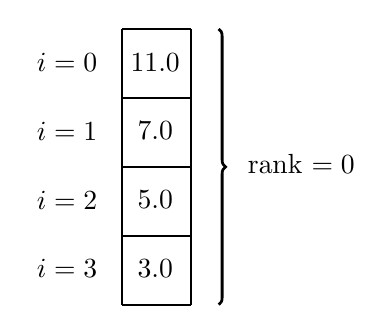
\begin{tikzpicture}[scale=3.5]
  \pgfmathsetmacro\fourth{1.0/4.0}
  \pgfmathsetmacro\xoff{0.12}
  \pgfmathsetmacro\yoff{0.12}
  \draw[xstep=\fourth,ystep=\fourth,black,thick] (0.0,0.0) grid (\fourth,1.0);
  \node at (-0.2,1.0-\yoff) {$i=0$};
  \node at (\xoff,1.0-\yoff) {$11.0$};
  \node at (-0.2,0.75-\yoff) {$i=1$};
  \node at (\xoff,0.75-\yoff) {$7.0$};
  \node at (-0.2,0.5-\yoff) {$i=2$};
  \node at (\xoff,0.5-\yoff) {$5.0$};
  \node at (-0.2,0.25-\yoff) {$i=3$};
  \node at (\xoff,0.25-\yoff) {$3.0$};
  \draw[decoration={brace,mirror,raise=5pt},decorate,line width=1pt] (0.3,0.0) -- (0.3,1.0);
  \node at (0.65,0.51) {rank $=0$};
\end{tikzpicture}
\bigskip
\caption{A sequential \pVec layout, all on rank $=0$ process.}
\label{fig:seqveclayout}
\end{marginfigure}

Suppose this sequence appears in a program called \texttt{myprogram.c}.  If the program is run sequentially on one process, i.e.~as
\begin{cline}
$ ./myprogram.c
\end{cline}
%$
then, at the end of the above create-assemble sequence, the storage of \texttt{x} looks like Figure \ref{fig:seqveclayout}.

However, if run as
\begin{cline}
$ mpiexec -n 2 ./myprogram.c
\end{cline}
%$
then the layout looks like Figure \ref{fig:mpitwoveclayout}.  In this case the argument \texttt{PETSC\_DECIDE} in \texttt{VecSetSizes()} is active because \PETSc \emph{decides} to put the first two entries of \texttt{x} on the rank $0$ process and the other two on the rank $1$ process. 

\begin{marginfigure}
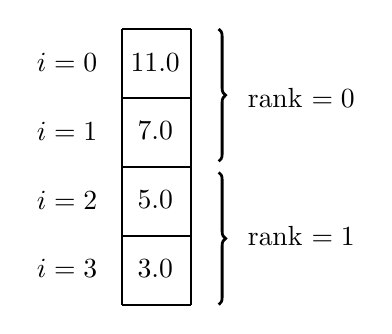
\begin{tikzpicture}[scale=3.5]
  \pgfmathsetmacro\fourth{1.0/4.0}
  \pgfmathsetmacro\xoff{0.12}
  \pgfmathsetmacro\yoff{0.12}
  \draw[xstep=\fourth,ystep=\fourth,black,thick] (0.0,0.0) grid (\fourth,1.0);
  \node at (-0.2,1.0-\yoff) {$i=0$};
  \node at (\xoff,1.0-\yoff) {$11.0$};
  \node at (-0.2,0.75-\yoff) {$i=1$};
  \node at (\xoff,0.75-\yoff) {$7.0$};
  \node at (-0.2,0.5-\yoff) {$i=2$};
  \node at (\xoff,0.5-\yoff) {$5.0$};
  \node at (-0.2,0.25-\yoff) {$i=3$};
  \node at (\xoff,0.25-\yoff) {$3.0$};
  \draw[decoration={brace,mirror,raise=5pt},decorate,line width=1pt] (0.3,0.52) -- (0.3,1.0);
  \node at (0.65,0.752) {rank $=0$};
  \draw[decoration={brace,mirror,raise=5pt},decorate,line width=1pt] (0.3,0.0) -- (0.3,0.48);
  \node at (0.65,0.251) {rank $=1$};
\end{tikzpicture}
\bigskip
\caption{A parallel \pVec layout on two processes.  Because we call ``\texttt{VecSetSizes(x,PETSC\_DECIDE,4)}'', \PETSc decides to split the storage in the middle.}
\label{fig:mpitwoveclayout}
\end{marginfigure}

Though in the current context it is completely artificial, one could override the ``\texttt{PETSC\_DECIDE}'' parallel layout by replacing the \texttt{VecSetSizes()} line with this block of code:
\begin{code}
PetscMPIInt rank;
MPI_Comm_rank(COMM,&rank);
if (rank == 0) {
  VecSetSizes(x,3,4);
} else if (rank == 1) {
  VecSetSizes(x,1,4);
} else {
  SETERRQ(COMM,1,"this code only works with size==2 communicators");
}
\end{code}
That is, we could specify the ``local size'' argument to \texttt{VecSetSizes()}, instead of using \texttt{PETSC\_DECIDE}.\sidenote{In fact such inflexible coding is rarely necessary.}  The resulting layout is shown in Figure \ref{fig:artificialmpitwoveclayout}.

In summary, the reader is allowed to think of a \PETSc \pVec as a one-dimensional C array with its range of indices and contents ``broken-up'' across the processes in the MPI communicator used in the \texttt{VecCreate()} command.

Parallel matrix objects \pMat, which are at some level conceived as 2D arrays, obviously require an additional choice regarding distribution.  But \PETSc makes this choice inside the implementation of \pMat.  Namely, \PETSc always stores ranges of complete rows on each process.  Said another way, conceptually at least, the column vectors which form the \pMat are stored like \pVecs.

While other storage formats are possible, the one usually used in this book is \emph{parallel compressed sparse row storage}, what \PETSc calls the \texttt{MATMPIAIJ} type.  That is, a range of rows is owned by each process (parallel row storage), and within each owned range of rows only the nonzero entries are stored (sparse), and furthermore the data structures store these nonzero entries contiguously in an array, with an additional contiguous index array (compressed).

\begin{marginfigure}
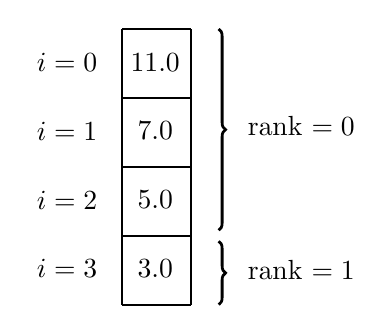
\begin{tikzpicture}[scale=3.5]
  \pgfmathsetmacro\fourth{1.0/4.0}
  \pgfmathsetmacro\xoff{0.12}
  \pgfmathsetmacro\yoff{0.12}
  \draw[xstep=\fourth,ystep=\fourth,black,thick] (0.0,0.0) grid (\fourth,1.0);
  \node at (-0.2,1.0-\yoff) {$i=0$};
  \node at (\xoff,1.0-\yoff) {$11.0$};
  \node at (-0.2,0.75-\yoff) {$i=1$};
  \node at (\xoff,0.75-\yoff) {$7.0$};
  \node at (-0.2,0.5-\yoff) {$i=2$};
  \node at (\xoff,0.5-\yoff) {$5.0$};
  \node at (-0.2,0.25-\yoff) {$i=3$};
  \node at (\xoff,0.25-\yoff) {$3.0$};
  \draw[decoration={brace,mirror,raise=5pt},decorate,line width=1pt] (0.3,0.27) -- (0.3,1.0);
  \node at (0.65,0.65) {rank $=0$};
  \draw[decoration={brace,mirror,raise=5pt},decorate,line width=1pt] (0.3,0.0) -- (0.3,0.23);
  \node at (0.65,0.125) {rank $=1$};
\end{tikzpicture}
\bigskip
\caption{A non-default parallel \pVec layout on two processes, by forcing local sizes to be not equal.}
\label{fig:artificialmpitwoveclayout}
\end{marginfigure}

For example, the following code creates and assembles a \pMat \texttt{A} with four rows and four columns:
% see testmatcreate.c
\begin{code}
Mat A;
PetscInt  i, j[3];
PetscReal v[3];

MatCreate(PETSC_COMM_WORLD,&A);
MatSetSizes(A,PETSC_DECIDE,PETSC_DECIDE,4,4);
MatSetFromOptions(A);
MatSetUp(A);

i = 0;
j[0] = 0;    j[1] = 1;
v[0] = 4.0;  v[1] = -1.0;
MatSetValues(A,1,&i,2,j,v,INSERT_VALUES);
i = 1;
j[0] = 0;    j[1] = 1;    j[2] = 2;
v[0] = -1.0; v[1] = 4.0;  v[2] = -1.0;
MatSetValues(A,1,&i,3,j,v,INSERT_VALUES);
i = 2;
j[0] = 1;    j[1] = 2;    j[2] = 3;
MatSetValues(A,1,&i,3,j,v,INSERT_VALUES);
i = 3;
j[0] = 2;    j[1] = 3;
MatSetValues(A,1,&i,2,j,v,INSERT_VALUES);

MatAssemblyBegin(A,MAT_FINAL_ASSEMBLY);
MatAssemblyEnd(A,MAT_FINAL_ASSEMBLY);
\end{code}
The method \texttt{MatSetValues()} sets a \emph{block} of values, and in this case we use it to set each row of the matrix.  Thus ``\texttt{1,\&i}'' arguments to \texttt{MatSetValues()} say ``we are setting one row, and look at the location of integer \texttt{i} for the (global) index.''  The ``\texttt{3,\&j}'' arguments, used in the \texttt{i} $=1,2$ rows, say ``we are setting three values in the row, and look at integer array \texttt{j} for the (global) indices.''

If the above lines appeared in \texttt{myprogram.c}, and if it was run
\begin{cline}
$ mpiexec -n 2 ./myprogram
\end{cline}
%$
then this \pMat would have the entries and layout shown in Figure \ref{fig:mpitwomatlayout}.

\begin{marginfigure}
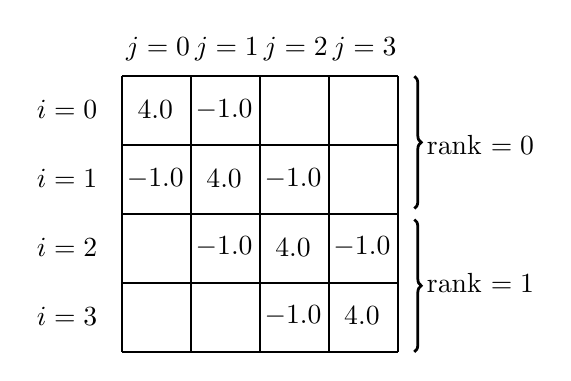
\begin{tikzpicture}[scale=3.5]
  \pgfmathsetmacro\fourth{1.0/4.0}
  \pgfmathsetmacro\xoff{0.12}
  \pgfmathsetmacro\yoff{0.12}
  \draw[xstep=\fourth,ystep=\fourth,black,thick] (0.0,0.0) grid (1.0,1.0);

  \node at (-0.2, 1.0-\yoff) {$i=0$};
  \node at (-0.2,0.75-\yoff) {$i=1$};
  \node at (-0.2, 0.5-\yoff) {$i=2$};
  \node at (-0.2,0.25-\yoff) {$i=3$};

  \node at ( 1.0-\xoff, 1.1) {$j=3$};
  \node at (0.75-\xoff, 1.1) {$j=2$};
  \node at ( 0.5-\xoff, 1.1) {$j=1$};
  \node at (0.25-\xoff, 1.1) {$j=0$};

  \node at (\xoff,1.0-\yoff) {$4.0$};
  \node at (0.25+\xoff,1.0-\yoff) {$-1.0$};

  \node at (\xoff,0.75-\yoff) {$-1.0$};
  \node at (0.25+\xoff,0.75-\yoff) {$4.0$};
  \node at (0.5+\xoff,0.75-\yoff) {$-1.0$};

  \node at (0.25+\xoff,0.5-\yoff) {$-1.0$};
  \node at (0.5+\xoff,0.5-\yoff) {$4.0$};
  \node at (0.75+\xoff,0.5-\yoff) {$-1.0$};

  \node at (0.5+\xoff,0.25-\yoff) {$-1.0$};
  \node at (0.75+\xoff,0.25-\yoff) {$4.0$};

  \draw[decoration={brace,mirror,raise=5pt},decorate,line width=1pt] (1.01,0.52) -- (1.01,1.0);
  \node at (1.3,0.752) {rank $=0$};
  \draw[decoration={brace,mirror,raise=5pt},decorate,line width=1pt] (1.01,0.0) -- (1.01,0.48);
  \node at (1.3,0.251) {rank $=1$};
\end{tikzpicture}
\bigskip
\caption{A parallel \pMat layout on two processes.  Blank entries are zeros, which are not stored because of ``compressed sparse'' storage.}
\label{fig:mpitwomatlayout}
\end{marginfigure}

We can have \PETSc show us the \pMat in different formats at the command line:
\begin{cline}
$ ./myprogram -mat_view
Mat Object: 1 MPI processes
  type: seqaij
row 0: (0, 4)  (1, -1)
row 1: (0, -1)  (1, 4)  (2, -1)
row 2: (1, -1)  (2, 4)  (3, -1)
row 3: (2, -1)  (3, 4)
$ ./myprogram -mat_view ::ascii_dense
Mat Object: 1 MPI processes
  type: seqaij
 4.00000e+00  -1.00000e+00  0.00000e+00  0.00000e+00
 -1.00000e+00  4.00000e+00  -1.00000e+00  0.00000e+00
 0.00000e+00  -1.00000e+00  4.00000e+00  -1.00000e+00
 0.00000e+00  0.00000e+00  -1.00000e+00  4.00000e+00
\end{cline}
The former view shows the compressed sparse storage, wherein only the nonzero values are shown, as pairs with column index and value, while the latter is a traditional (``dense'') display where zero values are shown.  In these cases the matrix was stored in \emph{serial} compressed sparse row format, the \texttt{MATSEQAIJ} type.

The result vector of a \pMat-\pVec product is, of course, a linear combination of the columns of the \pMat.  Thus, in practice, ``parallel row storage'' layout normally means two things:\begin{itemize}
\item \PETSc internally distributes the rows of the \pMat $A$ the same way as the entries of the intended output \pVec $b$, i.e.~if $Ax=b$ for some $x$, at least when \texttt{PETSC\_DECIDE} is used in setting the \pMat sizes, and
\item before \PETSc multiplies a matrix times a vector, \PETSc automatically communicates (``scatters'') the whole vector to each process.
\end{itemize}
After the scatter the \pMat-\pVec product is a local operation, requiring no further communication.

FIXME: assembly of \pMat a bit idiosyncratic; \texttt{MatSetValues()} sets a \emph{block} of values, not arbitrary inserts into sparse storage; need either MatXXXSetPreallocation() or MatSetUp() before MatGetOwnershipRange()


\section{Solve a linear system in \PETSc}

\cinputpartnostrip{c1matvec.c}{Initialize \PETSc and set up \pVecs and \pMat.}{I}{}{//ENDSETUP}{code:matvecpartone}

FIXME: emphasize that \texttt{MatGetOwnershipRange()} means that different processes are assembling different rows, unlike earlier example where all processes inserted all values

\cinputpartnostrip{c1matvec.c}{Assemble \pMat $A$.  Assemble right-hand side $b$ via exact solution to system.}{II}{//ENDSETUP}{//ENDASSEMBLY}{code:matvecparttwo}

\cinputpartnostrip{c1matvec.c}{Set up \pKSP.  Solve.  Finalize.}{III}{//ENDASSEMBLY}{//END}{code:matvecpartthree}

FIXME: show sparse and Matlab-format output for \texttt{A}, noting we get this at the \texttt{MatAssemblyEnd()} stage %$ ./c1matvec -a_mat_view ::ascii_matlab

FIXME: solve without choosing method

FIXME: show how to solve with Gaussian elimination


\section{A bit more numerical linear algebra}

Many methods other than Gauss elimination are possible for solving linear systems.  Usually these methods are iterative, and they often use the \emph{residual}.  By definition, if $\bu_0\in \RR^N$ is a vector then by the residual for $\bu_0$, as an estimate of the solution to equation \eqref{introsystem}, is the vector
\begin{equation}
\br_0 = \bb - A \bu_0. \label{residualdefn}
\end{equation}

Evaluating the residual for a known vector $\bu_0$ requires only applying $A$ to it, an $O(N^2)$ operation at most.  However, most discretization schemes for PDEs generate matrices $A$ that are \emph{sparse}, with many more zero entries than nonzeros, and often the number of nonzeros per row is independent of $N$.  In such cases the operation $A\bu_0$ can be implemented in $O(N)$ operations.

The \emph{Richardson iteration} is an example of an iterative method based on the residual.  If $\bu_0$ is an initial estimate of the solution then it simply adds a multiple $\omega$ of the residual at each step:
\begin{equation}
\bu_{k+1} = \bu_k + \omega (\bb - A \bu_k).  \label{introrichardson}
\end{equation}
If significantly fewer than $O(N^2)$ steps are needed to make $\bu_k$ an adequate approximation of the exact solution $\bu$, then the Richardson iteration can improve on Gauss elimination.  On the other hand, the Richardson iteration may not converge.

\newcommand{\rvect}[3]{\ensuremath{\bu_{#1} = \begin{bmatrix} #2 \\ #3 \end{bmatrix}}}

\medskip\noindent\hrulefill
\begin{example} Consider the linear system
\begin{equation}
A \bu
= \begin{bmatrix}
10 & -1 \\ -1 & 1
\end{bmatrix}
\begin{bmatrix} u_1 \\ u_2 \end{bmatrix}
= \begin{bmatrix} 8 \\ 1 \end{bmatrix}
= \bb
 \label{introexample}
\end{equation}
which has solution $\bu = [1\,\, 2]^\top$.  If we start with estimate $\bu_0 = [0\,\, 0]^\top$ then the unweighted ($\omega=1$) Richardson iteration \eqref{introrichardson} gives a sequence of vectors % see ../matlab/richardsonex.m
\begin{equation}
\rvect{0}{0}{0}, \rvect{1}{8}{1}, \rvect{2}{-63}{9}, \rvect{3}{584}{-62}, \dots
\end{equation}
This sequence is not heading toward the solution $\bu = [1\,\, 2]^\top$.
\end{example}
\noindent\hrulefill

If we rewrite \eqref{introrichardson} as
\begin{equation}
\bu_{k+1} = (I - \omega A) \bu_k + \omega \bb  \label{introrewriterichardson}
\end{equation}
then it is easy to believe that the ``size'' of the matrix $I-\omega A$ will determine whether $\lim_{k\to\infty} \bu_k$ exists, for generic starting vectors $\bu_0$.

To examine such questions, we recall the definitions of \emph{eigenvalue} and \emph{singular value}.  A complex number $\lambda \in \CC$ is an eigenvalue of a square matrix $B\in\RR^{N\times N}$ if there is a nonzero vector $\bv\in\CC^N$ so that $B \bv = \lambda \bv$.    The singular values are the square roots of the eigenvalues of the matrix $B^*B$.\sidenote{The matrix $B^*B$ is symmetric and positive-definite so its eigenvalues are nonnegative.}  Singular values are also geometrically-defined as the lengths of semi-axes of the ellipsoid in $\RR^N$ that results from applying $B$ to all vectors in the unit sphere of $\RR^N$ \citep{TrefethenBau}.

The set of all eigenvalues of $B$ is the \emph{spectrum} $\sigma(B)$ of $B$, and properties of matrices that can be described in terms of eigenvalues or singular values are generically called ``spectral properties.''  For example, recall that $\|B\|_2$ is equal to the largest singular value of $B$, while $\|B^{-1}\|_2$ is equal to the inverse of the smallest singular value of $B$.  The 2-norm condition number $\kappa(B)$ is the ratio of largest to smallest singular values,\sidenote{The condition number of $B$ well-visualized as the eccentricity of the ellipsoid we used in defining the singular values geometrically.}, and thus is a spectral property of $B$.

It is an easy exercise to show that the Richardson iteration \eqref{introrichardson} will converge if and only if all the eigenvalues of $B=I-\omega A$ are inside the unit circle.  Defining the \emph{spectral radius} $\rho(B)$ of a matrix $B$ as the maximum norm of the eigenvalues of $A$, we can describe the convergence of the Richardson iteration this way:
\begin{equation}
\text{\eqref{introrichardson} converges if and only if } \rho(I-\omega A) < 1. \label{introconvergethm}
\end{equation}
We can also show that $\rho(B) \le \|B\|_2$ so \eqref{introrewriterichardson} converges if $\|I-\omega A\|_2 < 1$, but this norm condition is merely sufficient, while \eqref{introconvergethm} is necessary and sufficient.

Other examples of iterative methods include the classical Jacobi and Gauss-Siedel iterations.  The most powerful methods generate optimal, in various senses \citep{TrefethenBau}, estimates $\bu_k$ which are each linear combinations of vectors $\bb,A\bb,A^2\bb,\dots,A^{k-1}\bb$.  These methods are collectively called \emph{Krylov space methods} because the span of these vectors is a Krylov space.  Typically the effectiveness of the iteration on a given matrix $A$ depends on the eigenvalues or singular values of $A$.  We use Krylov space methods in Chapter \ref{chap:structured} and all later Chapters.  Examples are conjugate gradients (CG) and minimum residual methods (e.g.~MINRES or GMRES) \citep{Greenbaum1997}.

There are many other systems which are equivalent to \eqref{introsystem}.  In fact, if $P\in\RR^{N\times N}$ is an invertible square matrix then the systems
\begin{equation}
(P^{-1} A) \bu = P^{-1} \bb \label{introleftpre}
\end{equation}
and
\begin{equation}
(A P^{-1}) (P\bu) = \bb \label{introrightpre}
\end{equation}
obviously have the same solution $\bu$ as \eqref{introsystem}.  However, matrices $P^{-1} A$ or $A P^{-1}$ may have different eigenvalues, condition numbers, and so on, namely different spectral properties, from $A$.  While the accuracy of the approximate solution $\bu$ cannot be improved beyond the $\kappa(A) \eps$ level---fact i) cannot be overcome in that sense---methods can indeed take advantage of better conditioning or other spectral properties to generate $\bu$ more quickly.  Especially if $P^{-1}$ is easy to apply\sidenote{The inverse matrix $P^{-1}$ is ``easy to apply'' exactly if the system $P\bv = \bc$ is easy to solve for $\bv$ in the sense of low computational cost.} then this can be an advantageous idea when trying to approximate $\bu$ quickly.  Equivalent systems \eqref{introleftpre} and \eqref{introrightpre} are referred to as \emph{preconditioned} systems, with \eqref{introleftpre} called \emph{left preconditioning} and \eqref{introrightpre} called \emph{right-preconditioning}.  Preconditioning can help in making our Richardson iteration example converge.  

\medskip\noindent\hrulefill
\begin{examplecont}  Suppose we use the diagonal matrix from  \eqref{introexample} as $P$:
\begin{equation}
P = \begin{bmatrix}
10 & 0 \\ 0 & 1
\end{bmatrix}.  \label{introP}
\end{equation}
Being diagonal, this $P$ is easy to invert and apply.  The preconditioned Richardson iteration using $P$, namely
\begin{equation}
\bu_{k+1} = \bu_k + \omega (P^{-1} \bb - P^{-1} A \bu_k),  \label{introprerichardson}
\end{equation}
is much better behaved.  With $\bu_0 = [0\,\, 0]^*$ again we get this sequence from \eqref{introprerichardson}:
\begin{equation}
\rvect{0}{0}{0}, \rvect{1}{0.8}{1.0}, \rvect{2}{0.9}{1.8}, \rvect{3}{0.98}{1.90}, \dots
\end{equation}
This sequence is apparently going to $\bu = [1\,\, 2]^*$.  Of course, the explanation is not hard to see; in this case
\begin{equation}
\rho(I-A) = -9.1, \qquad \rho(I-P^{-1} A) = 0.32.
\end{equation}
Convergence claim \eqref{introconvergethm} matches this bit of evidence.
\end{examplecont}
\noindent\hrulefill

Many iterative methods superior to the Richardson iteration are implemented in \PETSc.  We will use several of them, with choice of method only at run-time.


\caveat{But \Matlab is all you want if scale does not matter.}


\section{Exercises}

\renewcommand{\labelenumi}{\arabic{chapter}.\arabic{enumi}\quad}
\begin{enumerate}
\item Program \texttt{c1e.c} does a terrible job of load-balancing because the computation of the factorial $n!$ requires more flops when the process rank is larger.  Modify the code to balance the load almost perfectly, with exactly one multiply operation on each \texttt{rank>0} process, by using a blocking send and receive operations (\texttt{MPI\_Send(),MPI\_Recv()}) to pass the result of the last factorial to the next rank.  (\emph{Of course now we have a code that does a ridiculous amount of communication.})
% e1balanced.c
\item Modify \texttt{c1matvec.c} to read an integer option\sidenote{Use methods \texttt{PetscOptionsBegin()}, \texttt{PetscOptionsInt()}, and \texttt{PetscOptionsEnd()} so that \texttt{-help} output explains the option.} \texttt{-N} and form an $N\times N$ matrix, with $-2$ on the diagonal and $1$ on the super- and sub-diagonals as before.  (Choose any desired right-hand-side.)  Use \PETSc runtime options to estimate the condition number of the matrix for sample $N$ values; the online \PETSc FAQ page\sidenote{\texttt{www.mcs.anl.gov/petsc/documentation/faq.html}} will help with these options.
% see "How can I determine the condition number of a matrix?" on the PETSc FAQ page; "be sure to avoid restarts"
% -pc_type none -ksp_type gmres -ksp_monitor_singular_value -ksp_gmres_restart 1000
\end{enumerate} % chapter 1

%%%%%%%%%%


\chapter{2. Linear PDEs: structured grids}

We start with a cliched example, the Poisson problem, because it is the right place to start.  Though the Poisson problem is a cliche in applied mathematics, it gives us the opportunity to use \PETSc several different ways, starting here with building a structured grid using \PETSc \pDMDA, and solving in parallel using a \pKSP object.

\section{Poisson-Dirichlet problem}

\cinputpart{c2poisson.c}{Set up \pDMDA object.}{I}{//CREATEGRID}{//ENDCREATEGRID}{code:ctwopoissoncreategrid}

\cinputpart{c2poisson.c}{Fill matrix entries using \texttt{MatSetValuesStencil}.}{II}{//CREATEMATRIX}{//ENDCREATEMATRIX}{code:ctwopoissoncreatematrix}

\cinputpart{c2poisson.c}{Solve using \pKSP, and report on solution.}{III}{//SOLVE}{//ENDSOLVE}{code:ctwopoissonsolve}

\section{Runtime control of linear solver}

FIXME: basic Krylov theory

\section{Time-dependent heat equation}

FIXME: we WON'T do explicit, but it would look like ...

FIXME: use TS for backward-euler
 % chapter 2

%%%%%%%%%%


The cliched Poisson problem can be exploited some more.  It gives us the opportunity to use \PETSc for important tasks we have not yet seen, including reading an unstructured mesh into \PETSc \pVecs, symmetric implementation of boundary conditions, and explicit preallocation of a \pMat in parallel.

\section{Example: The Poisson problem}

Let $\Omega \subset \RR^d$ be a bounded (open) region.  Suppose its boundary $\partial\Omega$ is well-behaved, for instance that it is Lipschitz-continuous \citep[section 1.2]{Ciarlet2002} or even polygonal.  Suppose $\partial\Omega$ is decomposed into (measurable) disjoint subsets $\partial_D \Omega$ and $\partial_N \Omega$ whose union is the entire boundary $\partial \Omega$.  The \emph{Poisson problem}, in strong form and including nonhomogeneous Dirichlet and Neumann boundary conditions, is\marginnote{%
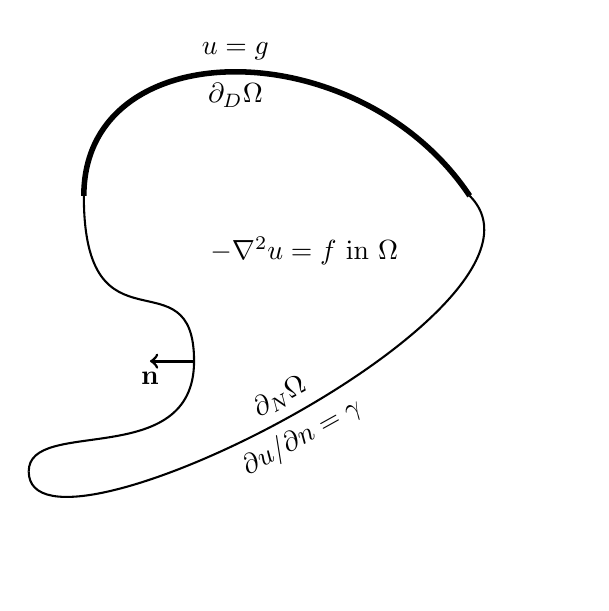
\begin{tikzpicture}[scale=0.7]
%\draw[gray,very thin] (-2,-6) grid (8,3);
\draw[line width=2pt] (0,0) .. controls (0,3) and (5,3) .. node[sloped,above] {$u=g$} node[sloped,below] {$\partial_D\Omega$} (7,0);
\draw[line width=0.75pt] (7,0) .. controls (9,-2) and (-1,-7) .. node[sloped,above] {$\partial_N\Omega$} node[sloped,below] {$\partial u/\partial n = \gamma$} (-1,-5);
\draw[line width=0.75pt] (-1,-5) .. controls (-1,-4) and (2,-5) .. (2,-3);
\draw[line width=0.75pt] (2,-3) .. controls (2,-1) and (0,-3) .. (0,0);
\draw[->,line width=1.0pt] (2,-3) -- (1.2,-3) node[below] {$\bn$}; % normal vector
\draw (4,-1) node {$- \grad^2 u = f$ in $\Omega$};
\end{tikzpicture}}
\begin{align}
- \grad^2 u &= f \quad \text{ on } \Omega, \label{poissonstrong} \\
u &= g \quad \text{ on } \partial_D \Omega, \notag \\
\frac{\partial u}{\partial n} &= \gamma \quad \text{ on } \partial_N \Omega \notag
\end{align}
where $\bn$ is the outward unit normal on $\partial \Omega$ and $\partial u/\partial n = \bn \cdot \grad u$.  The data of problem \eqref{poissonstrong}, besides the region $\Omega$ and its boundary, includes a \emph{source term} $f\in L^2(\Omega)$, \emph{Dirichlet data} $g\in L^2(\partial_N \Omega)$, and \emph{Neumann data} $\gamma\in L^2(\partial_N \Omega)$.

As \eqref{poissonstrong} is stated there may be no solution where ``$\grad^2 u$'' makes sense as a continuous function, even for polygonal regions, continuous boundary values, and continuous source functions.  In particular, there may be no $u\in C^2(\Omega)$ which is continuous up to the boundary (i.e.~$u\in C(\bar\Omega)$) and so that $\grad^2 u = f$.  There is, however, a solution if we change to a \emph{weak formulation}.\sidenote{A proof of this well-posedness claim is in \citet{Ciarlet2002} and in \citet{Evans2010}.  These are technicalities for us, however, as our goal is computational performance in cases where the Poisson problem is mathematically well-behaved and easily approximated.}  Furthermore, if $\partial_D \Omega$ has positive size, in an appropriate sense \citep[Theorem 1.2.1]{Ciarlet2002}, then the solution of the weak formulation is unique.  We will state the weak formulation after glossing the definitions of the needed function spaces.

Recalling $L^2(\Omega)$ is the space of all square-integrable real functions on $\Omega$, define
    $$H^1(\Omega) = \{u\in L^2(\Omega) \big| \grad u \text{ exists a.e.~and } \grad u \in L^2(\Omega)\},$$
which is a Sobolev space \citep{Evans2010}.  This space has two subsets we use, namely functions with value $g$ on $\partial_D \Omega$ and those with value $0$ on $\partial_D \Omega$, respectively, which we denote $H_g^1(\Omega)$ and $H_0^1(\Omega)$.  Note that $H_0^1(\Omega)$ is a linear subspace of $H^1(\Omega)$.  While $H_g^1(\Omega)$ is generally not a subspace (e.g.~because the zero function is not in it), it is an affine subspace, and we refer to both $H_g^1(\Omega)$ and $H_0^1(\Omega)$ as ``subspaces''.

To get to the weak formulation of the Poisson problem we suppose we already have a classical solution $u$ of \eqref{poissonstrong}.  Then we choose any $v\in H_0^1(\Omega)$, multiply the first equation in \eqref{poissonstrong} by $v$, and integrate by parts:
\begin{equation*}
\int_\Omega \grad u \cdot \grad v - \int_{\partial\Omega} \frac{\partial u}{\partial n} v = \int_\Omega f v.
\end{equation*}
Next\marginnote{%
{\color{red}Main ideas} of strong and weak formulations:\begin{itemize}
\item If $u \in H_g^1(\Omega)$ solves the strong form \eqref{poissonstrong} then it solves \eqref{poissonweak} also.
\item If $u \in H_g^1(\Omega)$ solves the weak form \eqref{poissonweak} then we accept it, by definition, as a solution of the Poisson problem.\end{itemize}} 
we use the other data, namely that $v=0$ on $\partial_D\Omega$ and that there is Neumann data $\gamma$ on $\partial_N\Omega$:
\begin{equation}
\int_\Omega \grad u \cdot \grad v = \int_\Omega f v + \int_{\partial_N\Omega} \gamma v\quad \text{ for any } v\in H_0^1(\Omega). \label{poissonweak}
\end{equation}

Equation \eqref{poissonweak} is the weak formulation of the Poisson problem.  Any $u \in H_g^1(\Omega)$ satisfying \eqref{poissonweak} is called a \emph{weak solution}.  A key observation is that $u$ itself incorporates the Dirichlet boundary condition, because it lives in $H_g^1(\Omega)$, while both the Neumann boundary data $\gamma$ and the source function $f$ appear in equation \eqref{poissonweak}.


\section{A finite element method (FEM) for the Poisson problem in the plane}

An FEM for the Poisson problem comes from requiring the weak formulation \eqref{poissonweak} to be true for $u$ in a much smaller, indeed finite-dimensional, subspace of $H_g^1(\Omega)$, and for test functions $v$ ranging over a finite-dimensional subspace of $H_0^1(\Omega)$.  In the ``Galerkin'' method here, these subspaces will be essentially the same.  We will build these subspaces, in the current example, using an unstructured triangulation on $\Omega\subset \RR^2$; from now on in this Chapter we restrict to $d=2$ dimensions.

Furthermore, to make our finite-dimensional spaces true subspaces of $H^1(\Omega)$---to make our FEM \emph{conforming}---we require that $\Omega$ be polygonal, with $\partial\Omega$ a closed polygon.  Segments of $\partial\Omega$ must have positive length, and be either entirely in $\partial_D\Omega$ or entirely in $\partial_N\Omega$.  We also assume $\partial_D\Omega$ is a closed set so that, at vertices of $\partial \Omega$ where the Dirichlet boundary and Neumann boundary meet, the vertex is Dirichlet.

By definition, a \emph{triangulation} is a finite set of non-overlapping, non-empty open triangles $\triangle_k\subset \RR^2$ which tile $\Omega$:
\begin{equation*}
\Th = \left\{\triangle_k \quad\Big|\quad \cup_k \overline{\triangle}_k = \overline{\Omega} \quad \text{ and} \quad \Omega_k \cap \Omega_l = \emptyset \text{ if } k\ne l\right\}.
\end{equation*}
We index the $K$ triangles in $\Th$ by $k=0,\dots,K-1$.  The $N$ vertices (nodes) in $\Th$ are indexed by $j=0,1,\dots,N-1$, with locations
\begin{equation*}
\bx_j = (x_j,y_j).
\end{equation*}
An example triangulation is shown in Figure \ref{fig:number-elements}.

\begin{marginfigure}
\input{samplepoly.1.tikz}
\caption{A triangulation $\Th$ with $K=22$ triangles (elements) numbered $k=0,1,\dots,K-1$ ({\color{red} red}) and $N=16$ nodes numbered $j=0,1,\dots,N-1$  ({\color{blue} blue}).  Nodes $\bx_0$, $\bx_1$, $\bx_2$, $\bx_3$ are in the Dirichlet boundary $\partial_D\Omega$.}
\label{fig:number-elements}
\end{marginfigure}

For now the reader can regard the subscript ``$h$'' in ``$\Th$'' as merely-traditional notation.  It denotes the typical or maximum size $h$ (e.g.~diameter) of the triangles, and it serves as a reminder that we want to approximate the solution in the limit $h\to 0$.  Also note that, in contrast to \citet{Elmanetal2005}, which we generally follow, and other references on the FEM or its implementation in languages like \Matlab, our indexing is zero-based.  This is so because we implement in C and we want to avoid any confusion when comparing text and codes.  Breaking long mathematical traditions, rows and columns of vectors and matrices will also have numbering starting with zero in this book.

We informally call the triangles \emph{elements}, though there is more to the definition of ``element.''  We are going to approximate the Poisson problem with $\Pone$ finite elements, which means that our finite-dimensional subspace contains only piecewise-linear functions which are linear on each triangle $\triangle_k$.

For each node $j$ there is a $\Pone$ basis function, or ``hat'' function, $\phi_j(x,y)$ which is linear on each triangle, continuous on all of $\overline{\Omega}$, and equal to one on only one node $j$:\marginnote{%
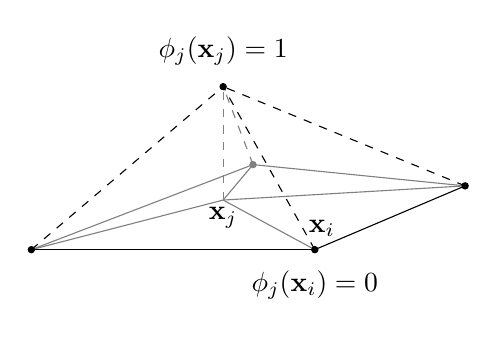
\begin{tikzpicture}[scale=0.9, z={(.707,.3)}]
    % (2,2,1) is top
    \draw[style=dashed] (0,0,0) -- (2,2,1); % to top from left
    \draw[style=dashed] (4,0,0) -- (2,2,1); %   ...  from front
    \draw[style=dashed] (4,0,3) -- (2,2,1); %   ...  from right
    \draw[color=gray, style=dashed] (0.3,0,4) -- (2,2,1); % from back
    \draw[color=gray, style=dashed] (2,0.4,1) -- (2,2,1); % from middle
    % draw base
    \draw (0,0,0) -- (4,0,0);
    \draw (4,0,0) -- (4,0,3);
    \draw[color=gray] (0,0,0) -- (0.3,0,4);
    \draw[color=gray] (0.3,0,4) -- (4,0,3);
    \draw[color=gray] (0,0,0) -- (2,0.4,1);
    \draw[color=gray] (2,0.4,1) -- (4,0,3);
    \draw[color=gray] (4,0,0) -- (2,0.4,1);
    \draw[color=gray] (2,0.4,1) -- (0.3,0,4);
    % draw \phi_j at nodes
    \filldraw (2,2,1) circle (1.25pt);
    \draw (2,2.5,1) node {$\phi_j(\bx_j)=1$};
    \draw (2,0.15,1) node {$\bx_j$};
    \filldraw (0,0,0) circle (1.25pt);
    \filldraw (4,0,0) circle (1.25pt);
    \draw (4,-0.5,0) node {$\phi_j(\bx_i)=0$};
    \draw (4.1,0.3,0) node {$\bx_i$};
    \filldraw (4,0,3) circle (1.25pt);
    \filldraw[color=gray] (0.3,0,4) circle (1.25pt);
\end{tikzpicture}
}%
\begin{equation*}
\phi_j(\bx_i) = \delta_{ij}.
\end{equation*}
The functions $\phi_j$ are in $H^1(\Omega)$, with piecewise-constant partial derivatives $\partial\phi_j/\partial x$ and $\partial\phi_j/\partial y$.  Also, the set $\{\phi_j\}_{j=0,\dots,N-1}$ is linearly-independent.  On each triangle, $\phi_j$ has three degrees of freedom, because on $\triangle_k$ there exist coefficients $A_k,B_k,C_k\in\RR$ so that
\begin{equation*}
\phi_j(\bx) = A_k + B_k x + C_k y \quad \text{ on } \triangle_k,
\end{equation*}
where $\bx = (x,y)$.

We can immediately use these basis functions to approximate the Dirichlet data $g$ and extend it to the region $\Omega$.  We will assume from now on that the Dirichlet boundary $\partial_D\Omega$ is closed, and index the $L$ nodes which are in the Dirichlet boundary by $\bx_{j_l} \in \partial_D\Omega$ for $l=0,\dots,L-1$.  (Figure \ref{fig:number-elements} shows an example with $L=4$ and $j_l=l$ for $l=0,1,2,3$, but any subset of boundary points can be Dirichlet as long as the index values $j_l$ are well-defined.)  Now we can define an extended interpolant $\hat g$ of $g$ as the function which has the correct value on the Dirichlet boundary nodes and which extends to all of $\Omega$ in a continuous and piecewise-linear way:
\begin{equation}
\hat g(\bx) = \sum_{l=0,\dots,L} g(\bx_{j_l}) \phi_{j_l}(\bx). \label{hatgdefine}
\end{equation}

By using $\hat g$ and the basis functions $\phi_j$, we can now describe three finite-dimensional subspaces of $H^1(\Omega)$:\sidenote{Traditionally, basis functions for $S_g^h$ are called the \emph{trial} functions, and basis functions for $S_0^h$ are called \emph{test} functions.  We will generally just use the labels ``$S_g^h$'' and ``$S_0^h$.''}
\begin{align*}
S^h &= \Span\{\phi_j \,\big|\, \text{ all } j\,\}, \\
S_0^h &= \Span\{\phi_j \,\big|\, \bx_j \notin \partial_D \Omega\} \subset S^h, \\
S_g^h &= S_0^h + \hat g \subset S^h.
\end{align*}
Then $\dim(S^h)=N$ while $\dim(S_0^h)=\dim(S_g^h)=N-L$, with $S_g^h$ only an affine subspace of $S^h$.

Our FEM requires that the weak formulation  \eqref{poissonweak} be true of $u_h\in S_g^h$ for all $v\in S_0^h$.  Thus we first write $u_h$ in the basis for $S_g^h$ using $N-L$ unknown coefficients $u_j$:
\begin{equation}
u_h(\bx) = \hat g(\bx) + \sum_{\bx_j \notin \partial_D \Omega} u_j\, \phi_j(\bx). \label{uhexpand}
\end{equation}
Then we require that the weak formulation hold for all $\phi_i$ in the basis of $S_0^h$.  That is, using definition \eqref{hatgdefine} and expansion \eqref{uhexpand}, we require
\begin{align}
\sum_{\bx_j \notin \partial_D \Omega} u_j \int_\Omega \grad \phi_j \cdot \grad \phi_i &= \int_\Omega f \phi_i + \int_{\partial_N\Omega} \gamma \phi_i \label{poissonfem} \\
&\qquad - \sum_{l=0,\dots,L} g(\bx_{j_l})  \int_\Omega \grad \phi_{j_l} \cdot \grad \phi_i \notag
\end{align}
for all $i$ such that $\bx_i \notin \partial_D \Omega$.  The coefficients $u_j$, for all $j$ such that $\bx_j \notin \partial_D \Omega$, are the unknowns in this equation.

Note that the support (i.e.~nonzero set) of $\phi_j$ includes only the node $\bx_j$ and all triangles (elements) $\triangle_k$ for which $\bx_j$ is a node of $\triangle_k$.  Thus the integral ``$\int_\Omega \grad \phi_j \cdot \grad \phi_i$'' in \eqref{poissonfem} is usually zero.  Specifically, it is zero if $\bx_i$ and $\bx_j$ are not both nodes of at least one triangle in the triangulation.


\section{Triangular meshes from \Triangle}

\PETSc itself does not include any tools for triangulating regions of the plane, sowe use the widely-available and easy-to-use \Triangle\sidenote{See \href{http://www.cs.cmu.edu/~quake/triangle.html}{www.cs.cmu.edu/$\sim$quake/ triangle.html} for documentation and source code. \Triangle may be available as a package in your operating system.} software \citep{Shewchuk1996} for this task.  \Triangle is both limited to planar regions and only capable of writing ASCII files.  Thus it is not a choice for performance, but of convenience.

\Triangle uses a simply-formatted ASCII file (extension \texttt{.poly}) as input to describe a polygonal region $\Omega$, and to indicate Dirichlet and Neumann portions of the boundary $\partial \Omega$.  For example, consider the input file \texttt{bump.poly} shown in Code \ref{code:bumppoly}.  This example polygon, a rectangle with a triangular bump in the base, is shown in Figure \ref{fig:bump-poly}.  It will reappear several times in this book as we solve more interesting PDEs on it.  The two apparently-unnecessary vertices introduced along the bottom help identify the Neumann part of the boundary, but note that \texttt{bump.poly} includes a Dirichlet/Neumann flag along each boundary segment.

\inputfromline{../c/ch8/bump.poly}{\CODELOC bump.poly}{A description of the boundary polygon in Figure \ref{fig:triangulation}, suitable for reading by \Triangle.}{16}{code:bumppoly}

The triangulation shown in Figure \ref{fig:triangulation} came from a single command which asks \Triangle to take \texttt{bump.poly} and generate a triangulation which has a polygon output file (option \texttt{-p}), relatively-uniform triangles (option \texttt{-q} for ``quality-checked'' \citep{Shewchuk1996}), and triangles with maximum area of $1.0$ (option \texttt{-a1.0}):
\begin{marginfigure}
\input{bump.poly.tikz}
\caption{The polygon described by \texttt{bump.poly} in Code \ref{code:bumppoly}.  The bold part is the closed Dirichlet boundary.  The lower boundary is Neumann, and has ``extra'' nodes to identify it as such.}
\label{fig:bump-poly}
\end{marginfigure}
\begin{cline}
$ triangle -pqa1.0 bump
\end{cline}
%$
This command generates three ASCII files, \texttt{bump.1.poly}, \texttt{bump.1.node}, and  \texttt{bump.1.ele}.  These files define the new (i.e.~refined relative to \texttt{bump.poly}) polygonal boundary, the nodes locations, and the elements in the triangulation, respectively.  For example, \texttt{bump.1.node} has the numbering and node locations shown in blue in Figure \ref{fig:triangulation}.

\Triangle includes a minimal visualization tool which shows the triangulation graphically.  The command
\begin{cline}
$ showme bump
\end{cline}
%$
displays the boundary polygon (from \texttt{bump.poly} or \texttt{bump.1.poly}) and the triangulation itself (\texttt{bump.1.node} and \texttt{bump.1.ele}).

\begin{figure}
\bigskip
% created by script tri2tikz.py command line:
%   ./tri2tikz.py --labelnodes --scale 2.0 --labeloffset 0.25 bump.1 bump.1.tikz
%
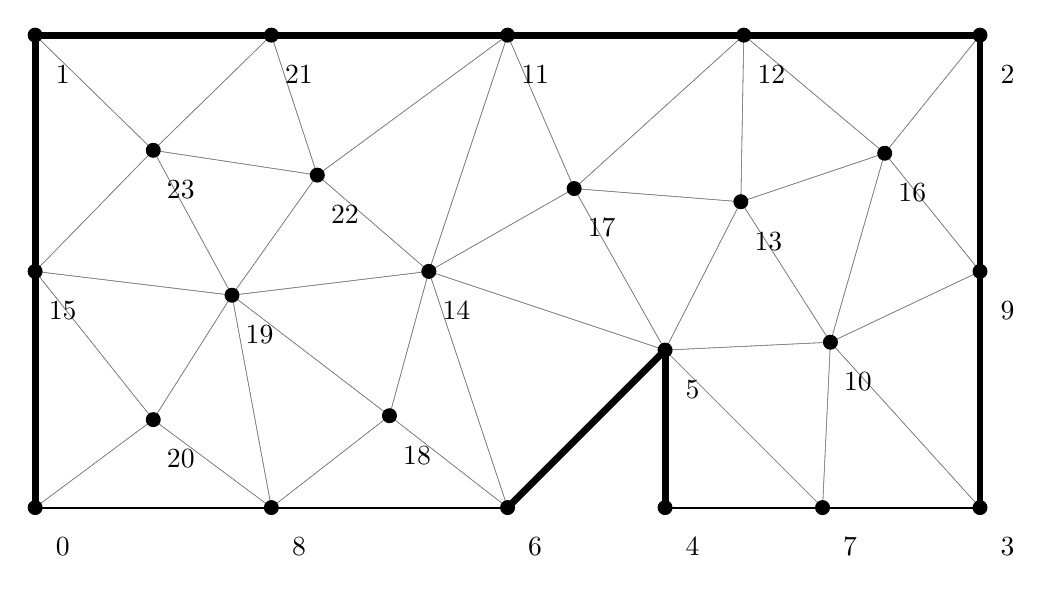
\begin{tikzpicture}[scale=2.000000]
  \draw[gray,very thin] (-1.500000,0.000000) -- (-2.250000,0.558372);
  \draw[gray,very thin] (-2.250000,0.558372) -- (-3.000000,0.000000);
  \draw[gray,very thin] (-3.000000,0.000000) -- (-1.500000,0.000000);
  \draw[gray,very thin] (-1.500000,0.000000) -- (0.000000,0.000000);
  \draw[gray,very thin] (0.000000,0.000000) -- (-0.750000,0.583333);
  \draw[gray,very thin] (-0.750000,0.583333) -- (-1.500000,0.000000);
  \draw[gray,very thin] (1.481325,1.942169) -- (0.422665,2.025778);
  \draw[gray,very thin] (0.422665,2.025778) -- (1.000000,1.000000);
  \draw[gray,very thin] (1.000000,1.000000) -- (1.481325,1.942169);
  \draw[gray,very thin] (-0.500000,1.500000) -- (0.000000,0.000000);
  \draw[gray,very thin] (0.000000,0.000000) -- (1.000000,1.000000);
  \draw[gray,very thin] (1.000000,1.000000) -- (-0.500000,1.500000);
  \draw[gray,very thin] (0.000000,3.000000) -- (-1.500000,3.000000);
  \draw[gray,very thin] (-1.500000,3.000000) -- (-1.208263,2.111158);
  \draw[gray,very thin] (-1.208263,2.111158) -- (0.000000,3.000000);
  \draw[gray,very thin] (2.000000,0.000000) -- (2.050000,1.050000);
  \draw[gray,very thin] (2.050000,1.050000) -- (1.000000,1.000000);
  \draw[gray,very thin] (1.000000,1.000000) -- (2.000000,0.000000);
  \draw[gray,very thin] (1.000000,0.000000) -- (2.000000,0.000000);
  \draw[gray,very thin] (2.000000,0.000000) -- (1.000000,1.000000);
  \draw[gray,very thin] (1.000000,1.000000) -- (1.000000,0.000000);
  \draw[gray,very thin] (2.394659,2.250000) -- (3.000000,1.500000);
  \draw[gray,very thin] (3.000000,1.500000) -- (3.000000,3.000000);
  \draw[gray,very thin] (3.000000,3.000000) -- (2.394659,2.250000);
  \draw[gray,very thin] (1.500000,3.000000) -- (0.422665,2.025778);
  \draw[gray,very thin] (0.422665,2.025778) -- (1.481325,1.942169);
  \draw[gray,very thin] (1.481325,1.942169) -- (1.500000,3.000000);
  \draw[gray,very thin] (2.050000,1.050000) -- (3.000000,0.000000);
  \draw[gray,very thin] (3.000000,0.000000) -- (3.000000,1.500000);
  \draw[gray,very thin] (3.000000,1.500000) -- (2.050000,1.050000);
  \draw[gray,very thin] (2.394659,2.250000) -- (2.050000,1.050000);
  \draw[gray,very thin] (2.050000,1.050000) -- (3.000000,1.500000);
  \draw[gray,very thin] (3.000000,1.500000) -- (2.394659,2.250000);
  \draw[gray,very thin] (-1.500000,3.000000) -- (-3.000000,3.000000);
  \draw[gray,very thin] (-3.000000,3.000000) -- (-2.250000,2.268853);
  \draw[gray,very thin] (-2.250000,2.268853) -- (-1.500000,3.000000);
  \draw[gray,very thin] (1.481325,1.942169) -- (1.000000,1.000000);
  \draw[gray,very thin] (1.000000,1.000000) -- (2.050000,1.050000);
  \draw[gray,very thin] (2.050000,1.050000) -- (1.481325,1.942169);
  \draw[gray,very thin] (3.000000,0.000000) -- (2.050000,1.050000);
  \draw[gray,very thin] (2.050000,1.050000) -- (2.000000,0.000000);
  \draw[gray,very thin] (2.000000,0.000000) -- (3.000000,0.000000);
  \draw[gray,very thin] (0.422665,2.025778) -- (1.500000,3.000000);
  \draw[gray,very thin] (1.500000,3.000000) -- (0.000000,3.000000);
  \draw[gray,very thin] (0.000000,3.000000) -- (0.422665,2.025778);
  \draw[gray,very thin] (2.394659,2.250000) -- (1.500000,3.000000);
  \draw[gray,very thin] (1.500000,3.000000) -- (1.481325,1.942169);
  \draw[gray,very thin] (1.481325,1.942169) -- (2.394659,2.250000);
  \draw[gray,very thin] (-1.750000,1.348485) -- (-0.750000,0.583333);
  \draw[gray,very thin] (-0.750000,0.583333) -- (-0.500000,1.500000);
  \draw[gray,very thin] (-0.500000,1.500000) -- (-1.750000,1.348485);
  \draw[gray,very thin] (-1.500000,0.000000) -- (-0.750000,0.583333);
  \draw[gray,very thin] (-0.750000,0.583333) -- (-1.750000,1.348485);
  \draw[gray,very thin] (-1.750000,1.348485) -- (-1.500000,0.000000);
  \draw[gray,very thin] (1.500000,3.000000) -- (2.394659,2.250000);
  \draw[gray,very thin] (2.394659,2.250000) -- (3.000000,3.000000);
  \draw[gray,very thin] (3.000000,3.000000) -- (1.500000,3.000000);
  \draw[gray,very thin] (2.050000,1.050000) -- (2.394659,2.250000);
  \draw[gray,very thin] (2.394659,2.250000) -- (1.481325,1.942169);
  \draw[gray,very thin] (1.481325,1.942169) -- (2.050000,1.050000);
  \draw[gray,very thin] (0.000000,3.000000) -- (-0.500000,1.500000);
  \draw[gray,very thin] (-0.500000,1.500000) -- (0.422665,2.025778);
  \draw[gray,very thin] (0.422665,2.025778) -- (0.000000,3.000000);
  \draw[gray,very thin] (1.000000,1.000000) -- (0.422665,2.025778);
  \draw[gray,very thin] (0.422665,2.025778) -- (-0.500000,1.500000);
  \draw[gray,very thin] (-0.500000,1.500000) -- (1.000000,1.000000);
  \draw[gray,very thin] (0.000000,0.000000) -- (-0.500000,1.500000);
  \draw[gray,very thin] (-0.500000,1.500000) -- (-0.750000,0.583333);
  \draw[gray,very thin] (-0.750000,0.583333) -- (0.000000,0.000000);
  \draw[gray,very thin] (-1.750000,1.348485) -- (-2.250000,2.268853);
  \draw[gray,very thin] (-2.250000,2.268853) -- (-3.000000,1.500000);
  \draw[gray,very thin] (-3.000000,1.500000) -- (-1.750000,1.348485);
  \draw[gray,very thin] (-3.000000,1.500000) -- (-3.000000,0.000000);
  \draw[gray,very thin] (-3.000000,0.000000) -- (-2.250000,0.558372);
  \draw[gray,very thin] (-2.250000,0.558372) -- (-3.000000,1.500000);
  \draw[gray,very thin] (-1.500000,0.000000) -- (-1.750000,1.348485);
  \draw[gray,very thin] (-1.750000,1.348485) -- (-2.250000,0.558372);
  \draw[gray,very thin] (-2.250000,0.558372) -- (-1.500000,0.000000);
  \draw[gray,very thin] (-3.000000,1.500000) -- (-2.250000,0.558372);
  \draw[gray,very thin] (-2.250000,0.558372) -- (-1.750000,1.348485);
  \draw[gray,very thin] (-1.750000,1.348485) -- (-3.000000,1.500000);
  \draw[gray,very thin] (0.000000,3.000000) -- (-1.208263,2.111158);
  \draw[gray,very thin] (-1.208263,2.111158) -- (-0.500000,1.500000);
  \draw[gray,very thin] (-0.500000,1.500000) -- (0.000000,3.000000);
  \draw[gray,very thin] (-0.500000,1.500000) -- (-1.208263,2.111158);
  \draw[gray,very thin] (-1.208263,2.111158) -- (-1.750000,1.348485);
  \draw[gray,very thin] (-1.750000,1.348485) -- (-0.500000,1.500000);
  \draw[gray,very thin] (-2.250000,2.268853) -- (-1.208263,2.111158);
  \draw[gray,very thin] (-1.208263,2.111158) -- (-1.500000,3.000000);
  \draw[gray,very thin] (-1.500000,3.000000) -- (-2.250000,2.268853);
  \draw[gray,very thin] (-3.000000,1.500000) -- (-2.250000,2.268853);
  \draw[gray,very thin] (-2.250000,2.268853) -- (-3.000000,3.000000);
  \draw[gray,very thin] (-3.000000,3.000000) -- (-3.000000,1.500000);
  \draw[gray,very thin] (-1.208263,2.111158) -- (-2.250000,2.268853);
  \draw[gray,very thin] (-2.250000,2.268853) -- (-1.750000,1.348485);
  \draw[gray,very thin] (-1.750000,1.348485) -- (-1.208263,2.111158);
  \draw[line width=2.5pt] (-3.000000,0.000000) -- (-3.000000,1.500000);
  \draw[line width=2.5pt] (-3.000000,3.000000) -- (-1.500000,3.000000);
  \draw[line width=2.5pt] (3.000000,3.000000) -- (3.000000,1.500000);
  \draw[line width=0.75pt] (3.000000,0.000000) -- (2.000000,0.000000);
  \draw[line width=0.75pt] (2.000000,0.000000) -- (1.000000,0.000000);
  \draw[line width=2.5pt] (1.000000,1.000000) -- (1.000000,0.000000);
  \draw[line width=2.5pt] (0.000000,0.000000) -- (1.000000,1.000000);
  \draw[line width=0.75pt] (0.000000,0.000000) -- (-1.500000,0.000000);
  \draw[line width=0.75pt] (-1.500000,0.000000) -- (-3.000000,0.000000);
  \draw[line width=2.5pt] (3.000000,1.500000) -- (3.000000,0.000000);
  \draw[line width=2.5pt] (0.000000,3.000000) -- (1.500000,3.000000);
  \draw[line width=2.5pt] (1.500000,3.000000) -- (3.000000,3.000000);
  \draw[line width=2.5pt] (-3.000000,1.500000) -- (-3.000000,3.000000);
  \draw[line width=2.5pt] (-1.500000,3.000000) -- (0.000000,3.000000);
  \draw (-2.825000,-0.250000) node {$0$};
  \filldraw (-3.000000,0.000000) circle (1.25pt);
  \draw (-2.825000,2.750000) node {$1$};
  \filldraw (-3.000000,3.000000) circle (1.25pt);
  \draw (3.175000,2.750000) node {$2$};
  \filldraw (3.000000,3.000000) circle (1.25pt);
  \draw (3.175000,-0.250000) node {$3$};
  \filldraw (3.000000,0.000000) circle (1.25pt);
  \draw (1.175000,-0.250000) node {$4$};
  \filldraw (1.000000,0.000000) circle (1.25pt);
  \draw (1.175000,0.750000) node {$5$};
  \filldraw (1.000000,1.000000) circle (1.25pt);
  \draw (0.175000,-0.250000) node {$6$};
  \filldraw (0.000000,0.000000) circle (1.25pt);
  \draw (2.175000,-0.250000) node {$7$};
  \filldraw (2.000000,0.000000) circle (1.25pt);
  \draw (-1.325000,-0.250000) node {$8$};
  \filldraw (-1.500000,0.000000) circle (1.25pt);
  \draw (3.175000,1.250000) node {$9$};
  \filldraw (3.000000,1.500000) circle (1.25pt);
  \draw (2.225000,0.800000) node {$10$};
  \filldraw (2.050000,1.050000) circle (1.25pt);
  \draw (0.175000,2.750000) node {$11$};
  \filldraw (0.000000,3.000000) circle (1.25pt);
  \draw (1.675000,2.750000) node {$12$};
  \filldraw (1.500000,3.000000) circle (1.25pt);
  \draw (1.656325,1.692169) node {$13$};
  \filldraw (1.481325,1.942169) circle (1.25pt);
  \draw (-0.325000,1.250000) node {$14$};
  \filldraw (-0.500000,1.500000) circle (1.25pt);
  \draw (-2.825000,1.250000) node {$15$};
  \filldraw (-3.000000,1.500000) circle (1.25pt);
  \draw (2.569659,2.000000) node {$16$};
  \filldraw (2.394659,2.250000) circle (1.25pt);
  \draw (0.597665,1.775778) node {$17$};
  \filldraw (0.422665,2.025778) circle (1.25pt);
  \draw (-0.575000,0.333333) node {$18$};
  \filldraw (-0.750000,0.583333) circle (1.25pt);
  \draw (-1.575000,1.098485) node {$19$};
  \filldraw (-1.750000,1.348485) circle (1.25pt);
  \draw (-2.075000,0.308372) node {$20$};
  \filldraw (-2.250000,0.558372) circle (1.25pt);
  \draw (-1.325000,2.750000) node {$21$};
  \filldraw (-1.500000,3.000000) circle (1.25pt);
  \draw (-1.033263,1.861158) node {$22$};
  \filldraw (-1.208263,2.111158) circle (1.25pt);
  \draw (-2.075000,2.018853) node {$23$};
  \filldraw (-2.250000,2.268853) circle (1.25pt);
\end{tikzpicture}

\caption{A FEM triangulation generated by \Triangle.  {\color{blue} Nodes} are labeled by $j=0,\dots,N-1$ with $N=24$ and {\color{red} elements} are labeled by $k=0,\dots,K-1$ with $K=32$.}
\label{fig:triangulation}
\end{figure}


\section{Getting a triangular mesh from ASCII files into a \PETSc \pVec}

The ASCII files produced by \Triangle produces are not in a good format for large meshes, but we will accept this for portability and readability.  We will, however, demonstrate how files are read in parallel, based on first doing a mundane and un-scalable task in \PETSc, namely reading the ASCII \Triangle files serially onto a single processor and writing out a binary file in \PETSc format.\sidenote{Furthermore we will focus on the scalability of the FEM solution process, once the mesh is loaded.}  The binary file both describes the mesh element-by-element and can be read in parallel.

The code \texttt{c3convert.c} does the conversion.  It is invoked, for the present purposes, by
\begin{cline}
$ c3convert -f bump.1
\end{cline}
%$
This reads ASCII files \texttt{bump.1.\{node,ele,poly\}} and writes a \PETSc-formatted binary file \texttt{bump.1.petsc}.

We will not show \texttt{c3convert.c}, but we summarize the high points.  First \PETSc is initialized and we get the rank of the current (MPI) process.  We only ask the first process (``rank zero'') in the MPI communicator to do any work.\sidenote{This code can be invoked ``\texttt{mpiexec -n NN c3convert}'', but it behaves as a serial code.}  This part of the code first reads the header information in the \texttt{.node} file, and allocates \PETSc \pVecs according.  We use \texttt{VecCreateSeq} to allocate the a sequential \pVec \texttt{vx}, which contains the $x$-coordinate of the nodes, only on the rank zero process.  Then \texttt{VecDuplicate} is used to allocate two more \pVecs with the same layout, \texttt{vy} and \texttt{vBT}.  This last \pVec will contain a flag $\{0,2,3\}$ for each node, where $0$ is an interior node, $2$ is a Dirichlet boundary node, and $3$ is a Neumann boundary node.

Then we read the node locations from the \texttt{.node} file.  The reading itself is done with the standard C library call \texttt{fscanf}.  Then \texttt{VecSetValues} is used to set one entry at a time.  After setting these values, which stores a list of entrys into an internal \PETSc dynamic data structure, we ask \PETSc to assemble the \pVecs.

The next part of \texttt{c3convert.c} reads boundary polygon information from the \texttt{.poly} file.  Each segment of the boundary polygon corresponds to two node indices.  We store the segments in a \pVec with blocksize 2.  Then we read the header information in the \texttt{.ele} file and allocates a \pVec called \texttt{vE} for the elements.  This part of the code is an important transformation of the data structures.  In fact, \texttt{vE} has block size 15,\sidenote{A \PETSc \pVec is designed to hold \texttt{PetscScalar} data types, i.e.~\texttt{double}.  So we are being quite wasteful for integer indices and boolean flags.} and, in contrast to the format from \Triangle, it contains all the information about each element that we need to do assemble the matrix equation.  Each of its blocks is the C \texttt{struct} shown in Code \ref{code:elementtype}.

\cinputraw{../c/ch8/readmesh.h}{extract from \texttt{\CODELOC readmesh.h}}{The \texttt{elementtype} struct.}{}{//STARTSTRUCT}{//ENDSTRUCT}{code:elementtype}

In the next part of \texttt{c3convert.c} we fill the \pVec for elements with all of the information read so far, including the node indices for each element which we read from the \texttt{.ele} file.  This stage is fundamentally serial, because we must look at the entire mesh to find the node coordinates and node/segment boundary type for each node and edge of each element.  In this part there is an important detail about triangulations, which affects the data structure for elements.  Namely, we cannot tell if an edge of an element is in the boundary just by whether both endpoints are in the boundary.  For example, the element (triangle) labeled ``5'' in Figure \ref{fig:triangulation} has an edge from node 5 (on the Dirichlet boundary) to node 7 (on the Neumann boundary).  But triangle 5 is \emph{not} a boundary element.  Thus we need to have list of flags for the boundary segments themselves.  Thus the \texttt{elementtype} structure above has both a boundary type for each node of each element and a boundary type for each edge of each element.

At this point we have the whole triangulation into \PETSc \pVecs.  The almost-last part of \texttt{c3convert.c} simply creates a \PETSc ``viewer'' and ``view'' all of the \pVecs which contain the mesh.  We will be able to reread these \pVecs in parallel, as long as we re-read them in the same order.  The final bit of \texttt{c3convert.c} checks if option \texttt{-check} is given, and if so we read back the binary file in parallel.  This part of \texttt{c3convert.c} calls two methods from a separate code (and re-used component) \texttt{readmesh.c} (Codes \ref{code:readmeshpartone} and \ref{code:readmeshparttwo}).

The first method \texttt{getmeshfile()} finds a \PETSc binary file from the \texttt{-f} option.  The other major method \texttt{readmesh()}, in Code \ref{code:readmeshparttwo}, creates and reads three \pVecs in parallel from it, using utility methods \texttt{createloadname()} and \texttt{getcheckmeshsizes()}.  Note that prefixes are set on each \pVec so that the block size is correctly read.

\cinputpart{readmesh.c}{\CODELOC}{Determine the filename of a \PETSc binary file that has a mesh.}{I}{//STARTGET}{//ENDGET}{code:readmeshpartone}

\cinputpart{readmesh.c}{\CODELOC}{Read the mesh in parallel from the file.}{II}{//STARTREADMESH}{//ENDREADMESH}{code:readmeshparttwo}


\section{Constructing the FEM linear system}

Now that we can get a triangulation into \PETSc, we can return to the finite-dimensional weak formulation \eqref{poissonfem}.  This linear system
\begin{equation}
A \bu = \bb, \label{poissonmatrix}
\end{equation}
has $A\in\RR^{N\times N}$ and $\bu,\bb\in\RR^N$, where $N$ is the number of nodes.  We will write a code which assembles $A$ and $\bb$ and solves for $\bu$.  \PETSc \pMat and \pVec objects store the problem, and we use a \pKSP object to solve it.

For ease of construction we include the node-wise Dirichlet conditions $u_j=g(\bx_j)$ as equations in this linear system, treating such $u_j$ as unknowns, so that the matrix has $N$ rows and columns if there are $N$ nodes in total.  Thus we define $A$ to have entries
\begin{equation}
a_{ij} = \int_\Omega \grad \phi_j \cdot \grad \phi_i \label{Aentryfem}
\end{equation}
if $\bx_i \notin \partial_D \Omega$ and $\bx_j \notin \partial_D \Omega$, while otherwise
\begin{equation*}
a_{ij} = \delta_{ij}.
\end{equation*}
Notice that we index rows and columns of matrices and vectors starting with zero,\sidenote{This follows C and \PETSc conventions, but is opposed to long-standing traditions about linear algebra!} and that $j=0,1,\dots,N-1$ in particular.

Observe that $A$ is \emph{symmetric}, $a_{ij}=a_{ji}$.  Furthermore $A$ is \emph{sparse}, that is, most entries are zero, at least for triangulations with more than a handful of triangles.  These facts affect the algorithms we choose when solving \eqref{poissonmatrix}.

For the right side of \eqref{poissonfem}, define the entries
\begin{equation}
    b_i = \int_\Omega f \phi_i + \int_{\partial_N\Omega} \gamma \phi_i - \sum_{l=0,\dots,L} g(\bx_{j_l})  \int_\Omega \grad \phi_{j_l} \cdot \grad \phi_i  \label{bentryfem}
\end{equation}
if $\bx_i \notin \partial_D \Omega$, while if $\bx_i \in \partial_D \Omega$ then
    $$b_i = g(\bx_{i}).$$

In practice we \emph{don't} initially build $A$ or $\bb$ as described above.  We start with a matrix $\tilde A$ and vector $\tilde \bb$ which have the same size as $A$ and $\bb$, respectively, but which ignore the Dirichlet boundary.  We don't even evaluate the function $g$.  All entries of $\tilde A$ are computed by the first formula above for $a_{ij}$, that is, the entries are
\begin{equation*}
\tilde a_{ij} = \int_\Omega \grad \phi_i \cdot \grad \phi_j
\end{equation*}
for all $i,j=0,1,\dots,N$.  Also the simpler right-hand side $\tilde \bb\in\RR^N$ has entries
    $$\tilde b_i = \int_\Omega f \phi_i + \int_{\partial_N\Omega} \gamma \phi_i$$
for all $i=0,1,\dots,N$.

This initial linear system $\tilde A\bu=\tilde \bb$ is (obviously) final in the case where there is no Dirichlet boundary (i.e.~$\partial_D \Omega=\emptyset$).  However, in this case $u=C$, where $C\in\RR$ is any constant value, solves $-\grad^2 u=0$ with $\partial u/\partial n = 0$ on the whole boundary $\partial_N \Omega = \partial \Omega$.  The Poisson problem then only determines the solution up to such an additive constant.  Because it does not have a unique solution, when solving \eqref{poissonmatrix} in this Neumann case we will have to inform \PETSc about the null space of constant functions.

In general, the next step is to edit $\tilde A$ in each Dirichlet row, that is, for each $i$ where $\bx_i \in \partial_D \Omega$.  For each such row we replace the whole row with the corresponding row of the identity, and also we replace $\tilde b_i$ with $b_i = g(\bx_i)$.  Furthermore, in each column $j$ for which $\bx_j \in \partial_D \Omega$, we move all entries $\tilde a_{ij}$ where $i$ is \emph{not} a Dirichlet row index over to the right-hand side, multiplied by the negative of the boundary value $g(\bx_{j})$.  We can write
\begin{equation}
    \tilde b_i \to \tilde b_i - g(\bx_{j}) \tilde a_{ij} \label{btransform}
\end{equation}
for these transformations.  After the completion of this ``editing'' stage we get $A$ and $\bb$.  Since this part of the matrix assembly is a key stage in our FEM codes, we now give a concrete example.

\medskip\noindent\hrulefill
\begin{example} Figure \ref{fig:squarefour} shows a triangulation of the unit square with five nodes.  The matrix $\tilde A$ has the following nonzero pattern; the zero entries are shown as spaces:\begin{marginfigure}
\input{squarefour.tikz}
\caption{A triangulation of a square with five nodes.  The top segment is the Dirichlet boundary.}
\label{fig:squarefour}
\end{marginfigure}%
\begin{equation*}
\tilde A = \begin{bmatrix}
\X & \X &    & \X & \X \\
\X & \X & \X &    & \X \\
   & \X & \X & \X & \X \\
\X &    & \X & \X & \X \\
\X & \X & \X & \X & \X
\end{bmatrix}.
\end{equation*}
Note $\tilde a_{ij}=0$ only where the integral $\int_\Omega \grad \phi_j \cdot \grad \phi_i$ is zero, a rare event in this small (coarse)-mesh case.  Now, because the $i=1,2$ nodes live in the (closed) Dirichlet boundary $\partial_D \Omega$, we highlight the $i=1,2$ rows and $j=1,2$ columns which will be edited:\marginnote{{\color{red} \textbf{Caution}}:  The first row or column of any matrix in this book is numbered ``$0$.''}
\begin{equation*}
\tilde A = \begin{bmatrix}
\X & \redX &    & \X & \X \\
\blueX & \blueX & \blueX &    & \blueX \\
   & \blueX & \blueX & \blueX & \blueX \\
\X &    & \redX & \X & \X \\
\X & \redX & \redX & \X & \X
\end{bmatrix}.
\end{equation*}
The underlined {\color{blue} blue} entries are changed to $0$ or $1$ so that these rows become rows of the identity; the old computed values $\tilde a_{ij}$ are tossed out.  The underlined {\color{red} red} entries, specifically the four entries $\tilde a_{01}$, $\tilde a_{32}$, $\tilde a_{41}$, and $\tilde a_{42}$, are moved over to the right side using transformation \eqref{btransform}; these $\tilde a_{ij}$ values get used.  The final linear system $A \bu = \bb$, is
\begin{equation*}
\begin{bmatrix}
\X & & & \X & \X \\
 & \,1\, & & & \\
 & & \,1\, & & \\
\X & & & \X & \X \\
\X & & & \X & \X
\end{bmatrix}
\begin{bmatrix}
u_0 \\
u_1 \\
u_2 \\
u_3 \\
u_4
\end{bmatrix}
=
\begin{bmatrix}
\tilde b_0 - g(\bx_1) \tilde a_{01} \\
g(\bx_1) \\
g(\bx_2) \\
\tilde b_3 - g(\bx_2) \tilde a_{32} \\
\tilde b_4 - g(\bx_1) \tilde a_{41} - g(\bx_2) \tilde a_{42}
\end{bmatrix}
\end{equation*}
\end{example}
\noindent\hrulefill

\bigskip


\section{Assembling the matrix equation, element by element}

An entry $\tilde a_{ij}$ of the initial matrix $\tilde A$ is not computed in one step.  Rather, we compute contributions to these entries from each element in turn; we ``loop over the elements.''  Furthermore we do it in parallel.  Recall that \texttt{c3convert.c} above creates a distributed \pVec called \texttt{E}, which is an array of elements of type \texttt{elementtype}, and \texttt{readmesh.c} reads it.

For the element-by-element assembly procedure we first define the integral over one triangle $\triangle_k$,
\begin{equation}
\text{\texttt{a(k,i,j)}} = \int_{\triangle_k} \grad \phi_i \cdot \grad \phi_. \label{aelementintegral}
\end{equation}
so that
    $$\tilde a_{ij} = \sum_k \phantom{.}\text{\texttt{a(k,i,j)}}.$$
Likewise we will compute
\begin{equation}
\text{\texttt{b(k,i)}} = \int_{\triangle_k} f \phi_i + \int_{\overline{\triangle}_k \cap \partial_N\Omega} \gamma \phi_i, \label{belementintegral}
\end{equation}
so that $\tilde b_i = \sum_{k} \;\text{\texttt{b(k,i)}}$.

If \texttt{E} denotes an array of \texttt{elementtype} then for each triangle $\triangle_k$ we can get the node index for each of its three vertices.  Using $q=0,1,2$ for these vertices,
    $$\text{\texttt{E[k].j[q]}} \in \{0,1,\dots,N-1\}.$$
Thus the element-by-element assembly of $\tilde A$ follows this pseudocode:
\begin{code}
A = 0                           // N x N sparse matrix with entries a(i,j)
b = 0                           // N x 1 column vector with entries b(i)
for k = 0 to K-1                // loop through all elements
    for q = 0 to 2
        i = E[k].j[q]           // row index
        for r = 0 to 2
            j = E[k].j[r]       // column index
            a(i,j) += a(k,q,r)  // add contribution from element k
            b(i)   += b(k,q)    // ditto
\end{code}
\medskip\noindent
Observe that on each triangle $\triangle_k$ we write ``\texttt{a(k,q,r)}'' for \texttt{a(k,i,j)}, by replacing the global indices $i,j$ by corresponding local node indices $q,r\in\{0,1,2\}$ for triangle $k$.

A standard approach to computing the element-wise integrals \texttt{a(k,q,r)} is to refer triangle $\triangle_k$ to a reference triangle $\triangle_\ast$ with vertices $(0,0),\,(1,0),\,(0,1)$, as shown in Figure \ref{fig:isoparametric}.  The linear map from $\triangle_\ast$ to $\triangle_k$ with vertices $(x_0,y_0),\,(x_1,y_1),\,(x_2,y_2)$, as shown in the Figure, is
\begin{align}
x(\xi,\eta) &= x_0 + (x_1-x_0) \xi + (x_2-x_0) \eta, \label{trianglemap} \\
y(\xi,\eta) &= y_0 + (y_1-y_0) \xi + (y_2-y_0) \eta. \notag
\end{align}

\begin{marginfigure}
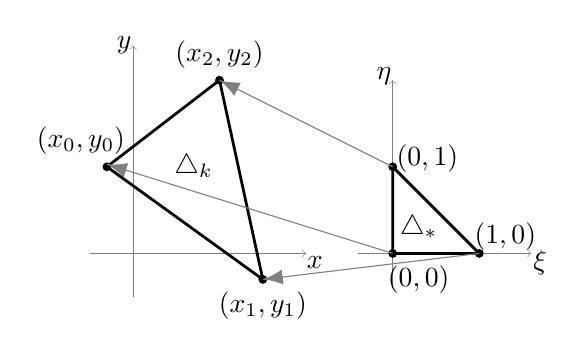
\begin{tikzpicture}[scale=1.1,
    decoration={
      markings,
      mark=at position 1 with {\arrow[scale=1.8,gray]{latex}};
    }]
% left x,y axes
    \draw[->, gray, very thin] (1.5,0) -- (4.0,0);
    \draw[->, gray, very thin] (2,-0.5) -- (2,2.4);
    \draw (4.1,-0.1) node {$x$};
    \draw (1.9,2.4) node {$y$};
    \filldraw (1.7,1) circle (1.25pt);    % (x_0,y_0)
    \filldraw (3.5,-0.3) circle (1.25pt); % (x_1,y_1)
    \filldraw (3.0,2.0) circle (1.25pt);  % (x_2,y_2)
    \draw (1.4,1.3) node {$(x_0,y_0)$};
    \draw (3.5,-0.6) node {$(x_1,y_1)$};
    \draw (3.0,2.3) node {$(x_2,y_2)$};
    \draw[line width=1pt] (1.7,1) -- (3.5,-0.3) -- (3.0,2.0) -- cycle;
    \draw (2.7,1.0) node {$\triangle_k$};
% right xi,eta axes
    \draw[->, gray, very thin] (4.6,0) -- (6.6,0);
    \draw[->, gray, very thin] (5,-0.4) -- (5,2.0);
    \draw (6.7,-0.1) node {$\xi$};
    \draw (4.9,2.05) node {$\eta$};
    \filldraw (5,0) circle (1.25pt);  % (0,0)
    \filldraw (6,0) circle (1.25pt);  % (1,0)
    \filldraw (5,1) circle (1.25pt);  % (0,1)
    \draw (5.3,-0.3) node {$(0,0)$};
    \draw (6.3,0.2) node {$(1,0)$};
    \draw (5.4,1.1) node {$(0,1)$};
    \draw[line width=1pt] (5,0) -- (6,0) -- (5,1) -- cycle;
    \draw (5.3,0.3) node {$\triangle_\ast$};
% arrows connecting nodes
    \draw[gray, postaction={decorate}] (5,0) -- (1.7,1.03);
    \draw[gray, postaction={decorate}] (6,0) -- (3.5,-0.3);
    \draw[gray, postaction={decorate}] (5,1) -- (3.0,2.0);
\end{tikzpicture}
\smallskip
\caption{Mapping of a triangle $\triangle_k$ from the reference triangle $\triangle_\ast$.}
\label{fig:isoparametric}
\end{marginfigure}

\noindent Furthermore, on $\triangle_\ast$ any linear function is a linear combination of these three local basis functions:
\begin{equation}
\chi_0(\xi,\eta) = 1-\xi-\eta, \qquad \chi_1(\xi,\eta) = \xi, \qquad \chi_2(\xi,\eta) = \eta. \label{chiformulas}
\end{equation}
On $\triangle_k$, each of the basis functions $\phi_q$ is the mapped version of the corresponding $\chi_q$:
\begin{equation}
\phi_q(x(\xi,\eta),y(\xi,\eta)) = \chi_q(\xi,\eta). \label{phichimap}
\end{equation}
From \eqref{trianglemap} and \eqref{phichimap} one can confirm that $\phi_q(x_r,y_r) = \delta_{qr}$.

Now is a good point at which to observe that the set of $\phi_j$, over all nodes $j=0,1,\dots,N$, is a partition of unity.  We can see this by switching to local node coordinate $q$ and using $\chi_0+\chi_1+\chi_2=1$, which is obvious from \eqref{chiformulas}.  That is, if $\bx \in \triangle_k$ then
\begin{equation}
   \sum_j \phi_j(\bx) = \sum_{q=0,1,2} \phi_q(\bx) = \sum_{q=0,1,2} \chi_q =1.  \label{partitionofunity}
\end{equation}

The Jacobian\sidenote{By definition, the \emph{Jacobian} $J=J(\bx)$ of a smooth map $F$ at a point $\bx$ is its linearization at $\bx$.  That is, if $\by=F(\bx)$ and $\by+\Delta\by = F(\bx+\Delta\bx)$ then $J(\bx)$ satisfies $\Delta \by = J(\bx) \Delta\bx + o(|\Delta\bx|)$.} of map \eqref{trianglemap} is
% CAUTION: Elman (1.37) uses "Jacobian" for the transpose of this, the true Jacobian (e.g. in Newton later)
\begin{equation}
J = \begin{bmatrix}
    \dfrac{\partial x}{\partial \xi} & \dfrac{\partial x}{\partial \eta} \\[1.0em]
    \dfrac{\partial y}{\partial \xi} & \dfrac{\partial y}{\partial \eta}
    \end{bmatrix}
    =
    \begin{bmatrix}
    x_1-x_0 & x_2-x_0 \\
    y_1-y_0 & y_2-y_0
    \end{bmatrix}.  \label{trianglejacobian}
\end{equation}
Recalling both the change-of-variables formula for integrals\sidenote{If $F$ is a smooth map from $\bx \in U$ to $\by \in F(U)$, $J$ is the Jacobian of $F$, and $g$ is integrable on $F(U)$, then $$\int_{F(U)} g(\by)\,d\by = \int_U g(F(\bx))\,|\det(J)|\,d\bx.$$} and the chain rule, by \eqref{phichimap} we can write
\begin{align}
\text{\texttt{a(k,q,r)}} &= \int_{\triangle_k} \grad\phi_q \cdot \grad\phi_r \label{elementcontrib} \\
   &= \int_{\triangle_k} \frac{\partial\phi_q}{\partial x} \frac{\partial\phi_r}{\partial x} + \frac{\partial\phi_q}{\partial y} \frac{\partial\phi_r}{\partial y} \; dx \, dy  \notag \\
   &= \int_{\triangle_\ast} \left(\frac{\partial \chi_q}{\partial \xi} \frac{\partial \xi}{\partial x} + \frac{\partial \chi_q}{\partial \eta} \frac{\partial \eta}{\partial x}\right) \left(\frac{\partial \chi_r}{\partial \xi} \frac{\partial \xi}{\partial x} + \frac{\partial \chi_r}{\partial \eta} \frac{\partial \eta}{\partial x}\right) \notag \\
   &\qquad\qquad + \left(\frac{\partial \chi_q}{\partial \xi} \frac{\partial \xi}{\partial y} + \frac{\partial \chi_q}{\partial \eta} \frac{\partial \eta}{\partial y}\right) \left(\frac{\partial \chi_r}{\partial \xi} \frac{\partial \xi}{\partial y} + \frac{\partial \chi_r}{\partial \eta} \frac{\partial \eta}{\partial y}\right) \; |\det(J)| \; d\xi \, d\eta. \notag
\end{align}
The last expression is the low point of this calculation.  From now on the formulas simplify because the integrand is \emph{constant} for the $\Pone$ elements here.  Indeed, by \eqref{trianglejacobian} we see $\det(J)$ is constant, but also the derivatives $\partial \chi_q/\partial\{\xi,\eta\}$ and $\partial\{\xi,\eta\}/\partial\{x,y\}$ are all constant because the functions in question are linear.

However, we need computable formulas for ``$\partial \xi/\partial x$'' and similar terms.  Again by the chain rule we can compute
\begin{equation*}
\begin{bmatrix}
    1 & 0 \\[0.2em]
    0 & 1
\end{bmatrix}
=\begin{bmatrix}
    \dfrac{\partial x}{\partial x} & \dfrac{\partial x}{\partial y} \\[1.0em]
    \dfrac{\partial y}{\partial x} & \dfrac{\partial y}{\partial y}
\end{bmatrix}
=
\begin{bmatrix}
    \dfrac{\partial x}{\partial \xi} & \dfrac{\partial x}{\partial \eta} \\[1.0em]
    \dfrac{\partial y}{\partial \xi} & \dfrac{\partial y}{\partial \eta}
\end{bmatrix}
\begin{bmatrix}
    \dfrac{\partial \xi}{\partial x} & \dfrac{\partial \xi}{\partial y} \\[1.0em]
    \dfrac{\partial \eta}{\partial x} & \dfrac{\partial \eta}{\partial y}
\end{bmatrix},
\end{equation*}
which is to say $I=J\; J^{-1}$.  On the other hand we can invert the $2\times 2$ matrix $J$ by hand to get
\begin{equation}
J^{-1}
= \frac{1}{\det(J)}
\begin{bmatrix}
    \dfrac{\partial y}{\partial \eta} & -\dfrac{\partial x}{\partial \eta} \\[1.0em]
    -\dfrac{\partial y}{\partial \xi} & \dfrac{\partial x}{\partial \xi}
\end{bmatrix}
= \frac{1}{\det(J)}
\begin{bmatrix}
    y_2-y_0 & x_0-x_2 \\
    y_0-y_1 & x_1-x_0
\end{bmatrix}.  \label{Jinverse}
\end{equation}
Now let $y_{20}=y_2-y_0$, $x_{02}=x_0-x_2$, $y_{01}=y_0-y_1$ and $x_{10}=x_1-x_0$.  In terms of these differences,
\begin{equation}
\begin{bmatrix}
    \dfrac{\partial \xi}{\partial x} & \dfrac{\partial \xi}{\partial y} \\[1.0em]
    \dfrac{\partial \eta}{\partial x} & \dfrac{\partial \eta}{\partial y}
\end{bmatrix}
= \frac{1}{\det(J)}
\begin{bmatrix}
    y_{20} & x_{02} \\
    y_{01} & x_{10}
\end{bmatrix} \label{dxietadxy}
\end{equation}
and
\begin{equation}
\det(J) = x_{10} y_{20} - y_{01} x_{02}. \label{detJ}
\end{equation}
Thus, by \eqref{elementcontrib}, \eqref{dxietadxy}, and \eqref{detJ}, and because the area of the reference triangle $\triangle_\ast$ is $1/2$\,, our element-wise contribution to $\tilde a_{ij}$ simplifies to
\begin{align}
\text{\texttt{a(k,q,r)}} = \frac{1}{2\; |\det(J)|} &\bigg[\left(\frac{\partial \chi_q}{\partial \xi} y_{20} + \frac{\partial \chi_q}{\partial \eta} y_{01}\right) \left(\frac{\partial \chi_r}{\partial \xi} y_{20} + \frac{\partial \chi_r}{\partial \eta} y_{01}\right) \label{elementcontribFINAL} \\
&\quad + \left(\frac{\partial \chi_q}{\partial \xi} x_{02} + \frac{\partial \chi_q}{\partial \eta} x_{10}\right) \left(\frac{\partial \chi_r}{\partial \xi} x_{02} + \frac{\partial \chi_r}{\partial \eta} x_{10}\right)\bigg]. \notag
\end{align}
Also note that
\begin{align}
\frac{\partial \chi_0}{\partial \xi} &= -1, & \frac{\partial \chi_1}{\partial \xi} &= 1, & \frac{\partial \chi_2}{\partial \xi} &= 0, \label{chiderivs} \\
\frac{\partial \chi_0}{\partial \eta} &= -1, & \frac{\partial \chi_1}{\partial \eta} &= 0, & \frac{\partial \chi_2}{\partial \eta} &= 1. \notag
\end{align}
Combining \eqref{elementcontribFINAL} and \eqref{chiderivs}, we know enough to write code to compute \texttt{a(k,q,r)}, and thus the entries in $\tilde A$.

To complete the code for the initial linear system $\tilde A \bu = \tilde\bb$ we also need to address the right-hand side $\tilde\bb$, that is, we need to compute the element-wise contribution \texttt{b(k,i)} in \eqref{belementintegral}.  We do these integrals by changing variables to the reference element, but we also only do the integrals approximately by quadrature.  This is because the data $f$ and $\gamma$ may have no analytically-computable integral, and because a modest error in evaluating the right side of the linear system can have only a small effect on the solution of the FEM linear system, which is, after all, only an approximation of the solution of the Poisson problem.

FIXME: in the homogeneous Neumann case ($\gamma=0$) we use midpoints of the edges of the triangles in our quadrature rule from \citet{Ciarlet2002}
\begin{align*}
\text{\texttt{b(k,q)}} &= \int_{\triangle_\ast} f\, \chi_q \; |\det(J)| \; d\xi \, d\eta \\
  &\approx \frac{|\det(J)|}{6} \left(\omega(0.5,0) + \omega(0.5,0.5) + \omega(0,0.5)\right)
\end{align*}
where $\omega(\xi,\eta) = f(x(\xi,\eta),y(\xi,\eta)) \chi_q(\xi,\eta)$.

%\section{Preallocate a \pMat}
%FIXME: figure showing parallel partition of elements
%\cinputpart{testprealloc.c}{Read mesh \pVecs from file.  Get row ownership range.}{I}{//STARTLOAD}{//ENDLOAD}{code:testpreallocpartone}
%\cinputpart{testprealloc.c}{Set up \pMat $A$ and actually preallocate it.  Fill it with junk entries so the pattern can be visualized.}{II}{//ENDLOAD}{//ENDTEST}{code:testpreallocparttwo}

\begin{comment}
From: Fande Kong <fdkong.jd@gmail.com>
To: PETSc users list <petsc-users@mcs.anl.gov>
Subject: Re: [petsc-users] Status on parallel mesh reader in DMPlex
> Message: 2
>Date: Fri, 18 Dec 2015 08:21:04 -0800
>From: Justin Chang <jychang48@gmail.com>
>To: petsc-users <petsc-users@mcs.anl.gov>
>Subject: [petsc-users] Status on parallel mesh reader in DMPlex

> Hi all,

>What's the status on the implementation of the parallel

I am actually developing a parallel loader. The loader has two steps:

(1) Use 1 core or several cores to read a sequential  mesh, and partition
it into $np$ parts using a partitioner, $np$ is the number of cores you
want to use to do a simulation. Usually, $np$ is large, for example, 10,000
cores. And then we write the partitioned data into the file system as a
HDF5 file.

(2) Load the partitioned data (HDF5 file) into $np$ cores in parallel.

This idea works pretty well for me at this point.  But, this loader is
not compatible with DMPlex now. However, I could change the code somehow,
If this idea is acceptable.

You could also implement it by yourself. It is not too bad.

>mesh reader/generator for DMPlex meshes? Is anyone actively working on
> this? If so is there a branch that I can peek into?

Parallel generator is highly nontrivial, I think. It is a very hard topic.

> Thanks,
> Justin
\end{comment}


\section{Solve the Poisson problem}

\cinputpart{poissontools.c}{\CODELOC}{Find Dirichlet rows, \texttt{INSERT\_VALUES} these, and call \texttt{MatAssemblyBegin/End} and \texttt{VecAssemblyBegin/End}.}{I}{//DIRICHLETROWS}{//ENDDIRICHLETROWS}{code:poissontoolsdirichlet}

\cinputpart{poissontools.c}{\CODELOC}{Start computing all other contributions element-by-element: Precompute all geometry of element and quadrature points.}{II}{//ASSEMBLEADDONE}{//ENDONE}{code:poissontoolsaddone}

\cinputpart{poissontools.c}{\CODELOC}{Compute all other contributions element-by-element including source $f$, Dirichlet columns using data $g$, and Neumann data $\gamma$.  Use \texttt{ADD\_VALUES} for these, and call \texttt{MatAssemblyBegin/End} and \texttt{VecAssemblyBegin/End}.}{III}{//ENDONE}{//ENDASSEMBLEADD}{code:poissontoolsaddtwo}

\cinputpart{poissontools.c}{\CODELOC}{Call \texttt{dirichletrows()} and \texttt{assembleadd()}.}{IV}{//FULLASSEMBLE}{//ENDFULLASSEMBLE}{code:poissontoolsassemble}


\cinputpart{poissonfem.c}{\CODELOC}{Read in mesh in parallel (i.e.~\pVec \texttt{E}) and create \pMat \texttt{A} and \pVec \texttt{b}.}{I}{//GETMESH}{//ENDMATVECCREATE}{code:cthreepoissongetmesh}

In the next part of the code (Code \ref{code:cthreepoissonchecks}) we do two basic checks on our assembly procedure, without solving a linear system.  First we check the construction of \texttt{A} by checking if constant functions are in the kernel when $\partial_D\Omega=\emptyset$.  In this check the data $f$, $g$, and $\gamma$ are all not used, and the boundary information in \texttt{E} is not used either.

\cinputpart{poissonfem.c}{\CODELOC}{Do two checks on the construction of the linear system.}{II}{//TWOCHECKS}{//ENDTWOCHECKS}{code:cthreepoissonchecks}

In the second check we verify the construction of $\bb$ in the case where $f\equiv 1$, $\gamma=0$, and $\partial_D\Omega=\emptyset$.  In this case, by formula \eqref{bentryfem} and observation \eqref{partitionofunity}, the sum of the entries of $\bb$ should be the area of the region:
   $$\sum_j b_j = \sum_j \int_\Omega 1\, \phi_j = \int_\Omega \sum_j \phi_j = |\Omega|.$$

\cinputpart{poissonfem.c}{\CODELOC}{Solve a Dirichlet problem for which we know the solution.}{III}{//SOLVEMANU}{//ENDSOLVEMANU}{code:cthreepoissonsolvemanu}


%\caveat{It works, but does it work well?}
 % chapter 3

%%%%%%%%%%


\chapter{4. Linear PDEs: multigrid}

We now make a key transition from Chapters 2 and 3.  Instead of writing code to assemble the matrix form of the problem on the grid initially chosen at runtime, and handing it to \pKSP for solution, we give a matrix-building code to \pKSP.  Then the \pKSP can choose the grid.  This gives the problem to a \PETSc \pKSP object in a way that allows it to do multigrid \citep{Briggsetal2000}.

\cinputpart{c4poisson.c}{Poisson problem on a structured grid again, but this time using \texttt{KSPSetComputeOperators()} so that multigrid is possible.}{I}{//MAIN}{//ENDMAIN}{code:multigridone}

\cinputpart{c4poisson.c}{This method builds the right-hand side.}{II}{//COMPUTERHS}{//ENDCOMPUTERHS}{code:multigridtwo}

\cinputpart{c4poisson.c}{This is the method handed to \texttt{KSPSetComputeOperators()}.}{III}{//COMPUTEJAC}{//ENDCOMPUTEJAC}{code:multigridthree}
 % chapter 4

%%%%%%%%%%


\chapter{Parallel scaling and performance}
\label{chap:scaling}

\section{Weak and strong scaling}

FIXME: define weak and strong scaling

\section{Assessing our performance with event-logging and \texttt{-log\_summary}}

\vspace{4cm}

FIXME: also we can put a structured grid in the unstructured code

\begin{marginfigure}
\input{mesh.1.tikz}
\caption{A structured triangulation of the unit square with $K=32$ triangles and $N=25$ nodes.  The entire boundary is Dirichlet in the problem we consider.}
\label{fig:structuredfem}
\end{marginfigure}

FIXME: use CG

\section{Classical preconditioners}

FIXME:  ILU?  block Jacobi and GS?

\section{Domain-decomposition preconditioners}

FIXME: ASM?

\section{Multigrid preconditioners}

FIXME: just show what we have already

FIXME: perhaps add 3D poisson

\section{Ideas}

FIXME: an idea that is most relevant to nonlinear problems: experimentation with linear solvers (i.e.~inside Newton) is obligatory because examples of linear systems can be found so that any solver comes out faster than any other \citep{Nachtigaletal1992} and examples of linear systems can be found so that well-known Krylov solvers like GMRES can be made to converge at any rate \citep{Greenbaumetal1996}

\caveat{But real-world PDEs are nonlinear.}
 % chapter 5

%%%%%%%%%%

\chapter{6. Nonlinear elliptic PDEs on structured grids}

\section{Newton's method}

\section{\textsc{SNES}}
% c4newton.c

\section{Example: a porous medium equation}

\section{Jacobians: actual and approximate}

\caveat{But it isn't scaling well yet.}


%%%%%%%%%%

\chapter{7. More run-time preconditioner composition}

\section{Indeterminant systems: Stokes}

\section{More preconditioners}

\caveat{But \PETSc should help with unstructured meshes too.}


%%%%%%%%%%

\chapter{8. Unstructured grids, the right way}

\section{\textsc{DMPlex}}

\caveat{But my PDE isn't really a PDE.  It has an inequality in it.}

%\caveat{But my PDE has ``$t$'' in it.}
%\chapter{7. Time-evolving problems}
%\section{\textsc{TS}}


%%%%%%%%%%

\chapter{9. PDEs with constraints}

\section{A variational inequality problem}


%%%%%%%%%%

\backmatter

\bibliography{book}
\bibliographystyle{plainnat}

\clearpage

\newcommand{\tblockeqncode}[3]{
\begin{tabular}[t]{l} #1: \\ \qquad {\small #2} \\ \quad {\large \underline{\texttt{#3}}} \end{tabular}
}
\newcommand{\tblockcode}[2]{
\begin{tabular}[t]{l} #1 \\ \quad {\large \underline{\texttt{#2}}} \end{tabular}
}
\newcommand{\tblock}[1]{
\begin{tabular}[t]{l} #1 \end{tabular}
}

\thispagestyle{empty}
\noindent \textsc{inside front cover:}

\vfill
\begin{center}
\hspace{-10mm}\begin{tabular}{rllll}
\toprule
Chapter 
    &\quad linear\quad
          &linear
                &\quad nonlinear\quad
                      &nonlinear \\ 
    &     &time-dependent
                &     &time-dependent \\
\midrule  \bigskip
1   &     &     &     &      \\ \bigskip
2   & \tblockeqncode{Poisson}{$-\grad^2 u = f$}{c2poisson.c}
          & \tblockeqncode{heat}{$u_t = \grad^2 u$}{c2heat.c}
                &     &      \\ \bigskip
3   & \tblockcode{Poisson}{c3poisson.c}
          &     &     &      \\ \bigskip
4   & \begin{minipage}[t]{35mm}
 \tblockcode{Poisson}{c4poisson.c}

 \tblockeqncode{advection-diffusion}{$\bv \cdot \grad u - \grad^2 u = f$}{c4ad.c}
\end{minipage}
          &     &     &      \\ \bigskip
5   &     &     &     &      \\ \bigskip
6   &     &     & \tblockeqncode{$p$-Laplace}{$\begin{matrix} -\Div\left(D \grad u\right) = f \\ D = |\grad u|^{p-2} \end{matrix}$}{c6plap.c}
                      & \tblockeqncode{porous}{$\begin{matrix} u_t = \Div\left(D \grad u\right) \\ D = u^{\gamma-1} \end{matrix}$}{c6porous.c} \\ \bigskip
7   & \tblockeqncode{Stokes}{$\begin{matrix} \Div u = 0 \\ \grad p = \grad^2 u \end{matrix}$}{c7stokes.c}
          &     &     &      \\ \bigskip
8   & \tblockcode{Poisson}{c8poisson.c}
          &     &     &      \\
    & \tblockcode{Stokes}{c8stokes.c}
          &     &     &      \\ \bigskip
9   &     &     & \tblockeqncode{obstacle}{$\begin{matrix} -\grad^2 u = f \\ u\ge \psi \end{matrix}$}{c9obstacle.c}
                      & \tblockeqncode{ice sheet}{$\begin{matrix} H_t = \Div\left(D \grad H\right) + f \\ D = H^{n+2} |\grad (H-b)|^{n-1} \\ H \ge 0\end{matrix}$}{c9ice.c} \\
\bottomrule
\end{tabular}
\end{center}
\vfill


\newpage\thispagestyle{empty}
\noindent \textsc{inside back cover:}

\vfill
\begin{center}
\begin{tabular}{rccccccc}
\toprule
Chapter 
    &\;\pVec\; &\;\pMat\;
                &\;\pKSP\; &\pDMDA
                            &\pDMPlex
                                  &\pSNES &\;\pTS\; \\
\midrule
1   & \XX & \XX & \XX &     &     &     &      \\
2   & \XX & \XX & \XX & \XX &     &     & \XX  \\
3   & \XX & \XX & \XX &     &     &     &      \\
4   & \gX & \gX & \XX & \XX &     &     &      \\
5   & \gX & \gX & \XX & \XX &     &     &      \\
6   & \gX & \gX & \XX & \XX &     & \XX & \XX  \\
7   & \gX & \gX & \gX & \XX &     & \XX &      \\
8   & \gX & \gX & \XX &     & \XX & \XX &      \\
9   & \gX & \gX & \gX & \XX &     & \XX &      \\
\bottomrule
\end{tabular}
\end{center}
\vfill

\end{document}
